\documentclass[10pt,a4paper]{article}
\usepackage[margin=0.75in]{geometry}
\usepackage[T1]{fontenc}
\usepackage[utf8]{inputenc}
\usepackage{lmodern,microtype,graphicx,booktabs,amsmath,xcolor,float,array}
\usepackage[font=small,labelfont=bf,skip=3pt]{caption}
\usepackage[shortlabels,inline]{enumitem}
\usepackage[hidelinks]{hyperref}
\usepackage{xurl}
\setlength{\parindent}{0pt}
\setlength{\parskip}{4pt}
\setlength{\emergencystretch}{3em}
\setlist{nosep,leftmargin=1.5em,itemsep=2pt}
\newcommand{\us}{$\mu$s}
% Generated by make_tables.py from the keys used in the TeX sources. Do not edit.
\expandafter\gdef\csname n@\detokenize{S:cases_completed}\endcsname{548}
\expandafter\gdef\csname n@\detokenize{S:cases_failed}\endcsname{1}
\expandafter\gdef\csname n@\detokenize{S:cases_notrun}\endcsname{103}
\expandafter\gdef\csname n@\detokenize{S:ext_pops}\endcsname{301}
\expandafter\gdef\csname n@\detokenize{S:ext_runs_max}\endcsname{6}
\expandafter\gdef\csname n@\detokenize{S:ext_runs_min}\endcsname{2}
\expandafter\gdef\csname n@\detokenize{S:ext_spread_max|.2f}\endcsname{2.98}
\expandafter\gdef\csname n@\detokenize{S:ext_spread_med|.2f}\endcsname{1.16}
\expandafter\gdef\csname n@\detokenize{S:ext_spread_n}\endcsname{301}
\expandafter\gdef\csname n@\detokenize{S:ext_spread_p90|.2f}\endcsname{1.30}
\expandafter\gdef\csname n@\detokenize{S:hit_speedup_max|.0f}\endcsname{162}
\expandafter\gdef\csname n@\detokenize{S:hit_speedup_min|.0f}\endcsname{45}
\expandafter\gdef\csname n@\detokenize{S:spdk_fabric_us|.0f}\endcsname{16}
\expandafter\gdef\csname n@\detokenize{S:th_matched}\endcsname{69}
\expandafter\gdef\csname n@\detokenize{S:th_matched_p50_faster}\endcsname{66}
\expandafter\gdef\csname n@\detokenize{S:th_matched_p50_slower}\endcsname{3}
\expandafter\gdef\csname n@\detokenize{S:th_matched_p99_slower}\endcsname{13}
\expandafter\gdef\csname n@\detokenize{S:th_mem_64k_hi|.2f}\endcsname{0.60}
\expandafter\gdef\csname n@\detokenize{S:th_mem_64k_lo|.2f}\endcsname{0.50}
\expandafter\gdef\csname n@\detokenize{S:th_mem_lower|.0f}\endcsname{25}
\expandafter\gdef\csname n@\detokenize{S:th_mem_pairs}\endcsname{27}
\expandafter\gdef\csname n@\detokenize{S:th_mem_ratio_hi|.2f}\endcsname{1.01}
\expandafter\gdef\csname n@\detokenize{S:th_mem_ratio_lo|.2f}\endcsname{0.50}
\expandafter\gdef\csname n@\detokenize{S:th_p50_slower}\endcsname{9}
\expandafter\gdef\csname n@\detokenize{S:th_p50_slower_mismatch}\endcsname{6}
\expandafter\gdef\csname n@\detokenize{S:th_p50_slower_tie}\endcsname{3}
\expandafter\gdef\csname n@\detokenize{S:th_p50_slower_tie_max|.2f}\endcsname{1.04}
\expandafter\gdef\csname n@\detokenize{S:th_pairs}\endcsname{80}
\expandafter\gdef\csname n@\detokenize{S:th_repeat_pairs}\endcsname{11}
\expandafter\gdef\csname n@\detokenize{S:th_repeat_ratio_hi|.2f}\endcsname{0.85}
\expandafter\gdef\csname n@\detokenize{S:th_repeat_ratio_lo|.2f}\endcsname{0.51}
\expandafter\gdef\csname n@\detokenize{S:th_ssd_pairs}\endcsname{1}
\expandafter\gdef\csname n@\detokenize{S:tl_exchange|.0f}\endcsname{105}
\expandafter\gdef\csname n@\detokenize{S:tl_span|.0f}\endcsname{383}
\expandafter\gdef\csname n@\detokenize{S:tl_waits_pct|.0f}\endcsname{52}
\expandafter\gdef\csname n@\detokenize{S:tl_waits|.0f}\endcsname{198}
\expandafter\gdef\csname n@\detokenize{S:tl_walpersist_pct|.0f}\endcsname{8}
\expandafter\gdef\csname n@\detokenize{S:tl_walpersist|.0f}\endcsname{31}
\expandafter\gdef\csname n@\detokenize{S:twin_p50_hi|.2f}\endcsname{1.05}
\expandafter\gdef\csname n@\detokenize{S:twin_p50_lo|.2f}\endcsname{0.89}
\expandafter\gdef\csname n@\detokenize{S:twin_p50_med|.2f}\endcsname{0.98}
\expandafter\gdef\csname n@\detokenize{S:twin_p99_hi|.1f}\endcsname{2.0}
\expandafter\gdef\csname n@\detokenize{S:twin_p99_hi|.2f}\endcsname{2.00}
\expandafter\gdef\csname n@\detokenize{S:twin_p99_lo|.2f}\endcsname{0.67}
\expandafter\gdef\csname n@\detokenize{S:twin_pairs}\endcsname{56}
\expandafter\gdef\csname n@\detokenize{S:vk_p50_slower}\endcsname{4}
\expandafter\gdef\csname n@\detokenize{S:vk_p999_slower}\endcsname{14}
\expandafter\gdef\csname n@\detokenize{S:vk_p99_slower}\endcsname{8}
\expandafter\gdef\csname n@\detokenize{S:vk_pairs}\endcsname{43}
\expandafter\gdef\csname n@\detokenize{S:xr_common}\endcsname{478}
\expandafter\gdef\csname n@\detokenize{S:xr_med:th_verbs|.2f}\endcsname{0.99}
\expandafter\gdef\csname n@\detokenize{S:xr_med:valkey_rdma|.2f}\endcsname{0.98}
\expandafter\gdef\csname n@\detokenize{S:xr_med:valkey_tcp|.2f}\endcsname{1.00}
\expandafter\gdef\csname n@\detokenize{S:xr_p10:th_verbs|.2f}\endcsname{0.60}
\expandafter\gdef\csname n@\detokenize{S:xr_p10:valkey_rdma|.2f}\endcsname{0.91}
\expandafter\gdef\csname n@\detokenize{S:xr_p10:valkey_tcp|.2f}\endcsname{0.98}
\expandafter\gdef\csname n@\detokenize{S:xr_p90:th_verbs|.2f}\endcsname{1.38}
\expandafter\gdef\csname n@\detokenize{S:xr_p90:valkey_rdma|.2f}\endcsname{1.03}
\expandafter\gdef\csname n@\detokenize{S:xr_p90:valkey_tcp|.2f}\endcsname{1.08}
\expandafter\gdef\csname n@\detokenize{amp:th_kernel:sealed_read:first_touch-scalar-c1-baseline:read:1024}\endcsname{5.0}
\expandafter\gdef\csname n@\detokenize{amp:th_kernel:sealed_read:first_touch-scalar-c1-baseline:read:256}\endcsname{17.1}
\expandafter\gdef\csname n@\detokenize{amp:th_kernel:sealed_read:first_touch-scalar-c1-baseline:read:64}\endcsname{65.5}
\expandafter\gdef\csname n@\detokenize{amp:th_kernel:sealed_read:first_touch-scalar-c1-baseline:read:65536}\endcsname{1.1}
\expandafter\gdef\csname n@\detokenize{amp:th_kernel:sealed_read:first_touch-scalar-c1-baseline:read:8192}\endcsname{1.5}
\expandafter\gdef\csname n@\detokenize{clientus:th_kernel:sealed_read:first_touch-scalar-c1-baseline:read:1024}\endcsname{14.6}
\expandafter\gdef\csname n@\detokenize{clientus:th_kernel:sealed_read:first_touch-scalar-c1-baseline:read:256}\endcsname{13.6}
\expandafter\gdef\csname n@\detokenize{clientus:th_kernel:sealed_read:first_touch-scalar-c1-baseline:read:8192}\endcsname{17.1}
\expandafter\gdef\csname n@\detokenize{cps:th_kernel:cold_os_cache:cold-os-large:read:65536}\endcsname{9,957}
\expandafter\gdef\csname n@\detokenize{cps:th_spdk:cold_os_cache:cold-os-large:read:65536}\endcsname{8,550}
\expandafter\gdef\csname n@\detokenize{cps:th_tcp:cold_os_cache:cold-os-large:read:65536}\endcsname{18,617}
\expandafter\gdef\csname n@\detokenize{cps:th_verbs:cold_os_cache:cold-os-large:read:65536}\endcsname{21,067}
\expandafter\gdef\csname n@\detokenize{cps:th_verbs:primary_rf1:write-concurrent:put:1024}\endcsname{51,467}
\expandafter\gdef\csname n@\detokenize{cps:valkey_rdma:primary_rf1:write-concurrent:put:1024}\endcsname{80,146}
\expandafter\gdef\csname n@\detokenize{dev:th_kernel:cold_os_cache:cold-os-large:read:65536|.1f}\endcsname{1.1}
\expandafter\gdef\csname n@\detokenize{dev:th_kernel:sealed_read:first_touch-scalar-c1-baseline:read:64}\endcsname{0.006}
\expandafter\gdef\csname n@\detokenize{dev:th_kernel:sealed_read:first_touch-scalar-c1-baseline:read:65536}\endcsname{1.008}
\expandafter\gdef\csname n@\detokenize{dev:th_kernel:sealed_read:first_touch-scalar-c1-baseline:read:8192}\endcsname{0.094}
\expandafter\gdef\csname n@\detokenize{dev:th_spdk:cold_os_cache:cold-os-large:read:65536|.1f}\endcsname{1.2}
\expandafter\gdef\csname n@\detokenize{dev:th_spdk:sealed_read:repeat_read-scalar-c1-baseline:read:65536}\endcsname{1.000}
\expandafter\gdef\csname n@\detokenize{dev:th_tcp:cold_os_cache:cold-os-large:read:65536|.1f}\endcsname{4.2}
\expandafter\gdef\csname n@\detokenize{dev:th_tcp:sealed_read:first_touch-scalar-c1-baseline:read:65536}\endcsname{0.542}
\expandafter\gdef\csname n@\detokenize{dev:th_tcp:sealed_read:first_touch-scalar-c1-baseline:read:8192}\endcsname{0.094}
\expandafter\gdef\csname n@\detokenize{dev:th_verbs:sealed_read:first_touch-scalar-c1-baseline:read:65536}\endcsname{1.001}
\expandafter\gdef\csname n@\detokenize{dev:th_verbs:sealed_read:first_touch-scalar-c1-baseline:read:8192}\endcsname{1.001}
\expandafter\gdef\csname n@\detokenize{devb:th_tcp:cold_os_cache:cold-os-large:read:65536}\endcsname{84,106}
\expandafter\gdef\csname n@\detokenize{devus:th_spdk:sealed_read:first_touch-scalar-c1-baseline:read:64}\endcsname{25.0}
\expandafter\gdef\csname n@\detokenize{devus:th_spdk:sealed_read:first_touch-scalar-c1-baseline:read:65536}\endcsname{87.2}
\expandafter\gdef\csname n@\detokenize{el:native:cold_os_cache:cold-os-large:read:65536}\endcsname{0.04}
\expandafter\gdef\csname n@\detokenize{el:th_kernel:cold_os_cache:cold-os-large:read:65536}\endcsname{0.41}
\expandafter\gdef\csname n@\detokenize{el:th_spdk:cold_os_cache:cold-os-large:read:65536}\endcsname{0.48}
\expandafter\gdef\csname n@\detokenize{gibs:th_kernel:primary_rf1:read-concurrent:read:65536}\endcsname{6.7}
\expandafter\gdef\csname n@\detokenize{gibs:th_spdk:primary_rf1:read-concurrent:read:65536}\endcsname{5.1}
\expandafter\gdef\csname n@\detokenize{gibs:th_verbs:primary_rf1:read-concurrent:read:65536}\endcsname{6.3}
\expandafter\gdef\csname n@\detokenize{gibs:valkey_rdma:primary_rf1:read-concurrent:read:65536}\endcsname{4.5}
\expandafter\gdef\csname n@\detokenize{hit:2:th_kernel:primary_rf1:point-mixed:read:1024}\endcsname{98}
\expandafter\gdef\csname n@\detokenize{hit:2:th_verbs:primary_rf1:point-mixed:read:1024}\endcsname{96}
\expandafter\gdef\csname n@\detokenize{hit:5:th_kernel:primary_rf1:point-mixed:read:1024}\endcsname{92}
\expandafter\gdef\csname n@\detokenize{hit:5:th_verbs:primary_rf1:point-mixed:read:1024}\endcsname{87}
\expandafter\gdef\csname n@\detokenize{initus:th_kernel:sealed_read:first_touch-scalar-c1-baseline:read:1024}\endcsname{23.8}
\expandafter\gdef\csname n@\detokenize{initus:th_kernel:sealed_read:first_touch-scalar-c1-baseline:read:256}\endcsname{23.2}
\expandafter\gdef\csname n@\detokenize{initus:th_kernel:sealed_read:first_touch-scalar-c1-baseline:read:8192}\endcsname{26.1}
\expandafter\gdef\csname n@\detokenize{initus:th_spdk:sealed_read:first_touch-scalar-c1-baseline:read:1024}\endcsname{48.7}
\expandafter\gdef\csname n@\detokenize{initus:th_spdk:sealed_read:first_touch-scalar-c1-baseline:read:64}\endcsname{40.9}
\expandafter\gdef\csname n@\detokenize{lower:p50:th_kernel/valkey_rdma:primary_rf1:read-concurrent:read:65536}\endcsname{34}
\expandafter\gdef\csname n@\detokenize{lower:p50:th_spdk/th_kernel:cold_os_cache:cold-os-large:read:65536}\endcsname{9}
\expandafter\gdef\csname n@\detokenize{lower:p50:th_verbs/valkey_rdma:primary_rf1:point-mixed:read:256}\endcsname{28}
\expandafter\gdef\csname n@\detokenize{lower:p50:th_verbs/valkey_rdma:primary_rf1:point-mixed:read:8192}\endcsname{25}
\expandafter\gdef\csname n@\detokenize{lower:p50:th_verbs/valkey_rdma:primary_rf1:read-concurrent:read:65536}\endcsname{29}
\expandafter\gdef\csname n@\detokenize{lower:p50:valkey_rdma/valkey_tcp:primary_rf1:read-concurrent:read:1024}\endcsname{19}
\expandafter\gdef\csname n@\detokenize{lower:p50:valkey_rdma/valkey_tcp:primary_rf1:write-concurrent:put:1024}\endcsname{6}
\expandafter\gdef\csname n@\detokenize{mean:th_kernel:cold_os_cache:cold-os-large:read:65536}\endcsname{1,562}
\expandafter\gdef\csname n@\detokenize{mean:th_spdk:cold_os_cache:cold-os-large:read:65536}\endcsname{1,827}
\expandafter\gdef\csname n@\detokenize{more:p50:th_kernel/native:cold_os_cache:cold-os-large:read:65536}\endcsname{34}
\expandafter\gdef\csname n@\detokenize{more:p50:th_spdk/native:cold_os_cache:cold-os-large:read:65536}\endcsname{21}
\expandafter\gdef\csname n@\detokenize{old:p50:th_kernel:sealed_read:repeat_read-batch32-c16-baseline:get_many:1024}\endcsname{40,031}
\expandafter\gdef\csname n@\detokenize{old:p50:th_verbs:primary_rf1:point-mixed:read:1024}\endcsname{22.7}
\expandafter\gdef\csname n@\detokenize{old:p50:th_verbs:primary_rf1:read-concurrent:read:1024}\endcsname{35.8}
\expandafter\gdef\csname n@\detokenize{old:p50:th_verbs:primary_rf1:read-many32:get_many:1024}\endcsname{1,126}
\expandafter\gdef\csname n@\detokenize{old:p50:th_verbs:primary_rf1:write-concurrent:put:1024}\endcsname{362}
\expandafter\gdef\csname n@\detokenize{p50:cassandra:primary_rf1:read-many32:get_many:1024}\endcsname{2,043}
\expandafter\gdef\csname n@\detokenize{p50:cassandra:primary_rf1:write-concurrent:put:1024}\endcsname{263}
\expandafter\gdef\csname n@\detokenize{p50:foundationdb:primary_rf1:write-concurrent:put:1024}\endcsname{986}
\expandafter\gdef\csname n@\detokenize{p50:garnet:primary_rf1:read-concurrent:read:1024}\endcsname{92.2}
\expandafter\gdef\csname n@\detokenize{p50:garnet:primary_rf1:write-concurrent:put:1024}\endcsname{144}
\expandafter\gdef\csname n@\detokenize{p50:kvrocks:primary_rf1:point-mixed:read:1024}\endcsname{50.0}
\expandafter\gdef\csname n@\detokenize{p50:kvrocks:primary_rf1:write-concurrent:put:1024}\endcsname{262}
\expandafter\gdef\csname n@\detokenize{p50:native:cold_os_cache:cold-os-large:read:65536}\endcsname{125}
\expandafter\gdef\csname n@\detokenize{p50:native:sealed_read:first_touch-scalar-c1-baseline:read:1024}\endcsname{0.88}
\expandafter\gdef\csname n@\detokenize{p50:native:sealed_read:first_touch-scalar-c1-baseline:read:256}\endcsname{0.62}
\expandafter\gdef\csname n@\detokenize{p50:native:sealed_read:first_touch-scalar-c1-baseline:read:8192}\endcsname{2.12}
\expandafter\gdef\csname n@\detokenize{p50:th_kernel:cold_os_cache:cold-os-large:read:65536}\endcsname{167}
\expandafter\gdef\csname n@\detokenize{p50:th_kernel:primary_rf1:point-mixed:read:1024}\endcsname{52.2}
\expandafter\gdef\csname n@\detokenize{p50:th_kernel:primary_rf1:read-concurrent:read:1024}\endcsname{55.9}
\expandafter\gdef\csname n@\detokenize{p50:th_kernel:primary_rf1:write-concurrent:put:1024}\endcsname{657}
\expandafter\gdef\csname n@\detokenize{p50:th_kernel:sealed_read:first_touch-scalar-c1-baseline:read:1024}\endcsname{36.5}
\expandafter\gdef\csname n@\detokenize{p50:th_kernel:sealed_read:first_touch-scalar-c1-baseline:read:256}\endcsname{35.0}
\expandafter\gdef\csname n@\detokenize{p50:th_kernel:sealed_read:first_touch-scalar-c1-baseline:read:8192}\endcsname{40.2}
\expandafter\gdef\csname n@\detokenize{p50:th_kernel:sealed_read:repeat_read-batch32-c16-baseline:get_many:1024}\endcsname{761}
\expandafter\gdef\csname n@\detokenize{p50:th_spdk:cold_os_cache:cold-os-large:read:65536}\endcsname{152}
\expandafter\gdef\csname n@\detokenize{p50:th_spdk:primary_rf1:point-mixed:read:1024}\endcsname{122}
\expandafter\gdef\csname n@\detokenize{p50:th_spdk:primary_rf1:read-concurrent:read:1024}\endcsname{71.7}
\expandafter\gdef\csname n@\detokenize{p50:th_spdk:primary_rf1:write-concurrent:put:1024}\endcsname{702}
\expandafter\gdef\csname n@\detokenize{p50:th_spdk:sealed_read:first_touch-scalar-c1-baseline:read:1024}\endcsname{59.2}
\expandafter\gdef\csname n@\detokenize{p50:th_spdk:sealed_read:first_touch-scalar-c1-baseline:read:64}\endcsname{54.3}
\expandafter\gdef\csname n@\detokenize{p50:th_spdk:sealed_read:first_touch-scalar-c1-baseline:read:65536}\endcsname{132}
\expandafter\gdef\csname n@\detokenize{p50:th_spdk:sealed_read:first_touch-scalar-c1-baseline:read:8192}\endcsname{99.7}
\expandafter\gdef\csname n@\detokenize{p50:th_tcp:cold_os_cache:cold-os-large:read:65536}\endcsname{610}
\expandafter\gdef\csname n@\detokenize{p50:th_tcp:coordinator_cache_configured:coordinator-cache:read:8192}\endcsname{0.88}
\expandafter\gdef\csname n@\detokenize{p50:th_tcp:primary_rf1:point-mixed:read:1024}\endcsname{41.5}
\expandafter\gdef\csname n@\detokenize{p50:th_tcp:primary_rf1:read-concurrent:read:1024}\endcsname{60.1}
\expandafter\gdef\csname n@\detokenize{p50:th_tcp:primary_rf1:read-many32:get_many:1024}\endcsname{840}
\expandafter\gdef\csname n@\detokenize{p50:th_tcp:primary_rf1:write-concurrent:put:1024}\endcsname{322}
\expandafter\gdef\csname n@\detokenize{p50:th_tcp:sealed_read:repeat_read-scalar-c1-baseline:read:1024}\endcsname{41.1}
\expandafter\gdef\csname n@\detokenize{p50:th_tcp:sealed_read:repeat_read-scalar-c1-baseline:read:256}\endcsname{39.4}
\expandafter\gdef\csname n@\detokenize{p50:th_verbs:cold_os_cache:cold-os-large:read:65536}\endcsname{519}
\expandafter\gdef\csname n@\detokenize{p50:th_verbs:coordinator_cache_configured:coordinator-cache:read:256}\endcsname{0.70}
\expandafter\gdef\csname n@\detokenize{p50:th_verbs:primary_rf1:point-mixed:put:1024}\endcsname{109}
\expandafter\gdef\csname n@\detokenize{p50:th_verbs:primary_rf1:point-mixed:read:1024}\endcsname{32.0}
\expandafter\gdef\csname n@\detokenize{p50:th_verbs:primary_rf1:read-concurrent:read:1024}\endcsname{45.0}
\expandafter\gdef\csname n@\detokenize{p50:th_verbs:primary_rf1:read-many32:get_many:1024}\endcsname{688}
\expandafter\gdef\csname n@\detokenize{p50:th_verbs:primary_rf1:read-many32:get_many:1024|.0f}\endcsname{688}
\expandafter\gdef\csname n@\detokenize{p50:th_verbs:primary_rf1:write-concurrent:put:1024}\endcsname{295}
\expandafter\gdef\csname n@\detokenize{p50:th_verbs:sealed_read:repeat_read-scalar-c1-baseline:read:1024}\endcsname{33.4}
\expandafter\gdef\csname n@\detokenize{p50:th_verbs:sealed_read:repeat_read-scalar-c1-baseline:read:64}\endcsname{31.6}
\expandafter\gdef\csname n@\detokenize{p50:tikv:primary_rf1:write-concurrent:put:1024}\endcsname{286}
\expandafter\gdef\csname n@\detokenize{p50:valkey_rdma:primary_rf1:point-mixed:put:1024}\endcsname{127}
\expandafter\gdef\csname n@\detokenize{p50:valkey_rdma:primary_rf1:point-mixed:read:1024}\endcsname{43.2}
\expandafter\gdef\csname n@\detokenize{p50:valkey_rdma:primary_rf1:point-mixed:read:256}\endcsname{43.6}
\expandafter\gdef\csname n@\detokenize{p50:valkey_rdma:primary_rf1:point-mixed:read:8192}\endcsname{50.6}
\expandafter\gdef\csname n@\detokenize{p50:valkey_rdma:primary_rf1:read-concurrent:read:1024}\endcsname{43.1}
\expandafter\gdef\csname n@\detokenize{p50:valkey_rdma:primary_rf1:read-many32:get_many:1024}\endcsname{321}
\expandafter\gdef\csname n@\detokenize{p50:valkey_rdma:primary_rf1:read-many32:get_many:1024|.0f}\endcsname{321}
\expandafter\gdef\csname n@\detokenize{p50:valkey_rdma:primary_rf1:write-concurrent:put:1024}\endcsname{173}
\expandafter\gdef\csname n@\detokenize{p999ms:th_kernel:cold_os_cache:cold-os-large:read:65536}\endcsname{336}
\expandafter\gdef\csname n@\detokenize{p999ms:th_spdk:cold_os_cache:cold-os-large:read:65536}\endcsname{428}
\expandafter\gdef\csname n@\detokenize{p99:native:cold_os_cache:cold-os-large:read:65536}\endcsname{219}
\expandafter\gdef\csname n@\detokenize{p99:th_kernel:cold_os_cache:cold-os-large:read:65536}\endcsname{913}
\expandafter\gdef\csname n@\detokenize{p99:th_spdk:cold_os_cache:cold-os-large:read:65536}\endcsname{376}
\expandafter\gdef\csname n@\detokenize{p99:th_tcp:sealed_read:first_touch-scalar-c1-baseline:read:256}\endcsname{67.6}
\expandafter\gdef\csname n@\detokenize{p99:th_tcp:sealed_read:first_touch-scalar-c1-baseline:read:64}\endcsname{65.1}
\expandafter\gdef\csname n@\detokenize{p99:th_verbs:primary_rf1:read-concurrent:read:1024}\endcsname{176}
\expandafter\gdef\csname n@\detokenize{p99:th_verbs:sealed_read:first_touch-scalar-c1-baseline:read:256}\endcsname{154}
\expandafter\gdef\csname n@\detokenize{p99:th_verbs:sealed_read:first_touch-scalar-c1-baseline:read:64}\endcsname{133}
\expandafter\gdef\csname n@\detokenize{p99:valkey_rdma:primary_rf1:read-concurrent:read:1024}\endcsname{92.5}
\expandafter\gdef\csname n@\detokenize{p99ms:garnet:primary_rf1:write-concurrent:put:1024}\endcsname{67}
\expandafter\gdef\csname n@\detokenize{p99ms:valkey_tcp:primary_rf1:read-many32:get_many:65536}\endcsname{213}
\expandafter\gdef\csname n@\detokenize{p99ms:valkey_tcp:primary_rf1:read-many32:get_many:8192}\endcsname{203}
\expandafter\gdef\csname n@\detokenize{ratio:p50:cassandra/th_verbs:primary_rf1:write-concurrent:put:1024}\endcsname{0.89}
\expandafter\gdef\csname n@\detokenize{ratio:p50:garnet/th_verbs:primary_rf1:write-concurrent:put:1024}\endcsname{0.49}
\expandafter\gdef\csname n@\detokenize{ratio:p50:kvrocks/th_verbs:primary_rf1:write-concurrent:put:1024}\endcsname{0.89}
\expandafter\gdef\csname n@\detokenize{ratio:p50:th_kernel/native:sealed_read:first_touch-scalar-c1-baseline:read:256|.0f}\endcsname{57}
\expandafter\gdef\csname n@\detokenize{ratio:p50:th_kernel/native:sealed_read:first_touch-scalar-c1-baseline:read:8192|.0f}\endcsname{19}
\expandafter\gdef\csname n@\detokenize{ratio:p50:th_kernel/valkey_rdma:primary_rf1:read-concurrent:read:65536}\endcsname{0.66}
\expandafter\gdef\csname n@\detokenize{ratio:p50:th_kernel/valkey_rdma:primary_rf1:read-many32:get_many:65536}\endcsname{0.88}
\expandafter\gdef\csname n@\detokenize{ratio:p50:th_kernel/valkey_rdma:primary_rf1:write-concurrent:put:1024}\endcsname{3.80}
\expandafter\gdef\csname n@\detokenize{ratio:p50:th_spdk/valkey_rdma:primary_rf1:write-concurrent:put:1024}\endcsname{4.06}
\expandafter\gdef\csname n@\detokenize{ratio:p50:th_tcp/th_kernel:cold_os_cache:cold-os-large:read:65536}\endcsname{3.64}
\expandafter\gdef\csname n@\detokenize{ratio:p50:th_tcp/th_spdk:cold_os_cache:cold-os-large:read:65536}\endcsname{4.02}
\expandafter\gdef\csname n@\detokenize{ratio:p50:th_tcp/valkey_tcp:primary_rf1:point-mixed:read:64}\endcsname{0.88}
\expandafter\gdef\csname n@\detokenize{ratio:p50:th_tcp/valkey_tcp:primary_rf1:point-mixed:read:65536}\endcsname{1.21}
\expandafter\gdef\csname n@\detokenize{ratio:p50:th_tcp/valkey_tcp:primary_rf1:point-mixed:read:8192}\endcsname{0.97}
\expandafter\gdef\csname n@\detokenize{ratio:p50:th_verbs/th_kernel:cold_os_cache:cold-os-large:read:65536}\endcsname{3.10}
\expandafter\gdef\csname n@\detokenize{ratio:p50:th_verbs/th_tcp:sealed_read:first_touch-scalar-c1-baseline:read:65536}\endcsname{1.52}
\expandafter\gdef\csname n@\detokenize{ratio:p50:th_verbs/th_tcp:sealed_read:first_touch-scalar-c1-baseline:read:8192}\endcsname{2.03}
\expandafter\gdef\csname n@\detokenize{ratio:p50:th_verbs/valkey_rdma:primary_rf1:point-mixed:put:1024}\endcsname{0.86}
\expandafter\gdef\csname n@\detokenize{ratio:p50:th_verbs/valkey_rdma:primary_rf1:point-mixed:put:256}\endcsname{0.87}
\expandafter\gdef\csname n@\detokenize{ratio:p50:th_verbs/valkey_rdma:primary_rf1:point-mixed:put:64}\endcsname{0.86}
\expandafter\gdef\csname n@\detokenize{ratio:p50:th_verbs/valkey_rdma:primary_rf1:point-mixed:put:65536}\endcsname{1.58}
\expandafter\gdef\csname n@\detokenize{ratio:p50:th_verbs/valkey_rdma:primary_rf1:point-mixed:put:8192}\endcsname{1.27}
\expandafter\gdef\csname n@\detokenize{ratio:p50:th_verbs/valkey_rdma:primary_rf1:point-mixed:read:256}\endcsname{0.72}
\expandafter\gdef\csname n@\detokenize{ratio:p50:th_verbs/valkey_rdma:primary_rf1:point-mixed:read:65536}\endcsname{0.85}
\expandafter\gdef\csname n@\detokenize{ratio:p50:th_verbs/valkey_rdma:primary_rf1:point-mixed:read:8192}\endcsname{0.75}
\expandafter\gdef\csname n@\detokenize{ratio:p50:th_verbs/valkey_rdma:primary_rf1:read-concurrent:read:65536}\endcsname{0.71}
\expandafter\gdef\csname n@\detokenize{ratio:p50:th_verbs/valkey_rdma:primary_rf1:read-many32:get_many:256}\endcsname{2.40}
\expandafter\gdef\csname n@\detokenize{ratio:p50:th_verbs/valkey_rdma:primary_rf1:read-many32:get_many:64}\endcsname{2.47}
\expandafter\gdef\csname n@\detokenize{ratio:p50:th_verbs/valkey_rdma:primary_rf1:read-many32:get_many:8192}\endcsname{1.59}
\expandafter\gdef\csname n@\detokenize{ratio:p50:th_verbs/valkey_rdma:primary_rf1:write-concurrent:put:64}\endcsname{1.53}
\expandafter\gdef\csname n@\detokenize{ratio:p50:th_verbs/valkey_rdma:primary_rf1:write-concurrent:put:65536}\endcsname{3.49}
\expandafter\gdef\csname n@\detokenize{ratio:p50:th_verbs/valkey_rdma:primary_rf1:write-concurrent:put:8192}\endcsname{2.18}
\expandafter\gdef\csname n@\detokenize{ratio:p50:tikv/th_verbs:primary_rf1:write-concurrent:put:1024}\endcsname{0.97}
\expandafter\gdef\csname n@\detokenize{ratio:p50:valkey_rdma/valkey_tcp:primary_rf1:offered-1000:put:1024}\endcsname{1.48}
\expandafter\gdef\csname n@\detokenize{ratio:p99:th_kernel/th_spdk:cold_os_cache:cold-os-large:read:65536}\endcsname{2.43}
\expandafter\gdef\csname n@\detokenize{ratio:p99:th_kernel/valkey_rdma:primary_rf1:read-concurrent:read:65536}\endcsname{0.54}
\expandafter\gdef\csname n@\detokenize{ratio:p99:th_tcp/th_kernel:cold_os_cache:cold-os-large:read:65536}\endcsname{4.06}
\expandafter\gdef\csname n@\detokenize{ratio:p99:th_tcp/valkey_tcp:primary_rf1:read-concurrent:read:64}\endcsname{2.03}
\expandafter\gdef\csname n@\detokenize{ratio:p99:th_tcp/valkey_tcp:primary_rf1:read-concurrent:read:8192}\endcsname{1.74}
\expandafter\gdef\csname n@\detokenize{ratio:p99:th_verbs/valkey_rdma:primary_rf1:point-mixed:put:1024}\endcsname{1.39}
\expandafter\gdef\csname n@\detokenize{ratio:p99:th_verbs/valkey_rdma:primary_rf1:point-mixed:put:64}\endcsname{1.34}
\expandafter\gdef\csname n@\detokenize{ratio:p99:th_verbs/valkey_rdma:primary_rf1:read-concurrent:read:64}\endcsname{1.96}
\expandafter\gdef\csname n@\detokenize{ratio:p99:th_verbs/valkey_rdma:primary_rf1:read-concurrent:read:65536}\endcsname{1.05}
\expandafter\gdef\csname n@\detokenize{ratio:p99:th_verbs/valkey_rdma:primary_rf1:read-concurrent:read:8192}\endcsname{1.99}
\expandafter\gdef\csname n@\detokenize{rej:cassandra:10000}\endcsname{30}
\expandafter\gdef\csname n@\detokenize{rej:foundationdb:50000}\endcsname{29,074}
\expandafter\gdef\csname n@\detokenize{rej:garnet:10000}\endcsname{9,725}
\expandafter\gdef\csname n@\detokenize{rej:garnet:50000}\endcsname{195,417}
\expandafter\gdef\csname n@\detokenize{rej:th_kernel:50000}\endcsname{16,587}
\expandafter\gdef\csname n@\detokenize{rej:th_spdk:50000}\endcsname{18,507}
\expandafter\gdef\csname n@\detokenize{rej:th_tcp:50000}\endcsname{7,600}
\expandafter\gdef\csname n@\detokenize{rej:tikv:50000}\endcsname{2}
\expandafter\gdef\csname n@\detokenize{rej:valkey_rdma:50000}\endcsname{2,131}
\expandafter\gdef\csname n@\detokenize{rm:0474:admit_us}\endcsname{66}
\expandafter\gdef\csname n@\detokenize{rm:0474:group_gap_us}\endcsname{116}
\expandafter\gdef\csname n@\detokenize{rm:0474:groups_per_call|.1f}\endcsname{4.7}
\expandafter\gdef\csname n@\detokenize{rm:0474:preflight_us}\endcsname{134}
\expandafter\gdef\csname n@\detokenize{rm:0474:submit_wait_us}\endcsname{265}
\expandafter\gdef\csname n@\detokenize{rm:0483:submit_wait_us}\endcsname{95}
\expandafter\gdef\csname n@\detokenize{rmcoord:0474}\endcsname{83}
\expandafter\gdef\csname n@\detokenize{rmcoord:0483}\endcsname{60}
\expandafter\gdef\csname n@\detokenize{rmpct:0093:flight_us}\endcsname{74}
\expandafter\gdef\csname n@\detokenize{rmpct:0474:flight_us}\endcsname{17}
\expandafter\gdef\csname n@\detokenize{rmpct:0483:flight_us}\endcsname{40}
\expandafter\gdef\csname n@\detokenize{stage:0011:profile:exchange}\endcsname{49.7}
\expandafter\gdef\csname n@\detokenize{stage:0011:profile:server_handler}\endcsname{10.1}
\expandafter\gdef\csname n@\detokenize{stage:0041:profile:exchange}\endcsname{37.7}
\expandafter\gdef\csname n@\detokenize{stage:0041:profile:server_handler}\endcsname{9.5}
\expandafter\gdef\csname n@\detokenize{stage:0282:profile:write_profile_storage_persist_wal_file_ns}\endcsname{29.5}
\expandafter\gdef\csname n@\detokenize{stage:0346:live_nvmeof:control_ns}\endcsname{160.8}
\expandafter\gdef\csname n@\detokenize{stage:0346:live_nvmeof:cq_ns}\endcsname{34.8}
\expandafter\gdef\csname n@\detokenize{stage:0346:live_nvmeof:frontier_file_ns}\endcsname{93.4}
\expandafter\gdef\csname n@\detokenize{stage:0346:live_nvmeof:frontier_namespace_ns}\endcsname{61.1}
\expandafter\gdef\csname n@\detokenize{stage:0346:live_nvmeof:persistence_ns}\endcsname{203.5}
\expandafter\gdef\csname n@\detokenize{stage:0346:live_nvmeof:wal_persistence_ns}\endcsname{35.8}
\expandafter\gdef\csname n@\detokenize{stage:0347:live_nvmeof:control_ns}\endcsname{164.7}
\expandafter\gdef\csname n@\detokenize{stage:0347:live_nvmeof:cq_ns}\endcsname{50.2}
\expandafter\gdef\csname n@\detokenize{stage:0347:live_nvmeof:frontier_file_ns}\endcsname{96.1}
\expandafter\gdef\csname n@\detokenize{stage:0347:live_nvmeof:frontier_namespace_ns}\endcsname{60.5}
\expandafter\gdef\csname n@\detokenize{stage:0347:live_nvmeof:persistence_ns}\endcsname{184.6}
\expandafter\gdef\csname n@\detokenize{stage:0347:live_nvmeof:wal_persistence_ns}\endcsname{14.9}
\expandafter\gdef\csname n@\detokenize{stagecount:0282:pre_completion_gate:write_durable_batches}\endcsname{4,096}
\expandafter\gdef\csname n@\detokenize{stagecount:0282:pre_completion_gate:write_durable_receipt_publication_blocked_batches}\endcsname{2,013}
\expandafter\gdef\csname n@\detokenize{stagecount:0283:authority:history_loads}\endcsname{2,760}
\expandafter\gdef\csname n@\detokenize{stagecount:0348:authority:history_loads}\endcsname{11}
\expandafter\gdef\csname n@\detokenize{stagecount:0349:authority:history_loads}\endcsname{11}
\expandafter\gdef\csname n@\detokenize{stagecount:0448:authority:history_loads}\endcsname{2,757}
\expandafter\gdef\csname n@\detokenize{tlbucket:w2_competing0}\endcsname{7}
\expandafter\gdef\csname n@\detokenize{tlbucket:w2_competing8}\endcsname{120}
\expandafter\gdef\csname n@\detokenize{tlbucket:w3_competing0}\endcsname{13}
\expandafter\gdef\csname n@\detokenize{tlbucket:w3_competing8}\endcsname{138}
\expandafter\gdef\csname n@\detokenize{tlcorr:w1}\endcsname{0.81}
\expandafter\gdef\csname n@\detokenize{tlcorr:w2}\endcsname{0.88}
\expandafter\gdef\csname n@\detokenize{tlcorr:w3}\endcsname{0.88}
\expandafter\gdef\csname n@\detokenize{tlowner:batches_per_owner_record|.1f}\endcsname{2.5}
\expandafter\gdef\csname n@\detokenize{wrtk:native:primary_rf1:write-concurrent:put:1024}\endcsname{1.9}
\expandafter\gdef\csname n@\detokenize{wrtk:th_kernel:primary_rf1:write-concurrent:put:1024}\endcsname{49.9}
\expandafter\gdef\csname n@\detokenize{wrtk:th_verbs:primary_rf1:write-concurrent:put:1024}\endcsname{17.7}
\expandafter\gdef\csname n@\detokenize{xratio:cps:th_verbs:primary_rf1:read-concurrent:valkey_rdma:primary_rf1:read-concurrent:read:65536}\endcsname{1.41}
\expandafter\gdef\csname n@\detokenize{xratio:p50:th_verbs:primary_rf1:read-concurrent:th_verbs:primary_rf1:point-mixed:read:1024}\endcsname{1.41}
\expandafter\gdef\csname n@\detokenize{xratio:p50:th_verbs:primary_rf1:write-concurrent:th_verbs:primary_rf1:point-mixed:put:1024}\endcsname{2.71}
\expandafter\gdef\csname n@\detokenize{xratio:p50:valkey_rdma:primary_rf1:read-concurrent:valkey_rdma:primary_rf1:point-mixed:read:1024}\endcsname{1.00}
\expandafter\gdef\csname n@\detokenize{xratio:p50:valkey_rdma:primary_rf1:write-concurrent:valkey_rdma:primary_rf1:point-mixed:put:1024}\endcsname{1.36}

\newcommand{\N}[1]{\ifcsname n@\detokenize{#1}\endcsname\csname n@\detokenize{#1}\endcsname\else\errmessage{Missing number #1}\fi}
% Generated by make_tables.py. Do not edit.
\newcommand{\RC}[3]{\N{#1:#2:primary_rf1:read-concurrent:read:#3}}
\newcommand{\WC}[3]{\N{#1:#2:primary_rf1:write-concurrent:put:#3}}
\newcommand{\MR}[3]{\N{#1:#2:primary_rf1:read-many32:get_many:#3}}
\newcommand{\WB}[3]{\N{#1:#2:primary_rf1:write-batch32:put_batch:#3}}
\newcommand{\PR}[3]{\N{#1:#2:primary_rf1:point-mixed:read:#3}}
\newcommand{\PP}[3]{\N{#1:#2:primary_rf1:point-mixed:put:#3}}
\newcommand{\FT}[3]{\N{#1:#2:sealed_read:first_touch-scalar-c1-baseline:read:#3}}
\newcommand{\RR}[3]{\N{#1:#2:sealed_read:repeat_read-scalar-c1-baseline:read:#3}}
\newcommand{\FS}[3]{\N{#1:#2:sealed_read:first_touch-scalar-c16-baseline:read:#3}}
\newcommand{\CO}[3]{\N{#1:#2:cold_os_cache:cold-os-large:read:#3}}
\newcommand{\CC}[3]{\N{#1:#2:coordinator_cache_configured:coordinator-cache:read:#3}}

\newcommand{\inference}{\textbf{[INFERENCE]}}
\newcommand{\runs}{Tidehunter and Native: one run; other stores: median of \N{S:ext_runs_min} to \N{S:ext_runs_max} runs}
\begin{document}
\begin{center}
{\LARGE\bfseries Distributed Tidehunter}\\[3pt]
{\large Full-matrix Google Cloud campaign: results, comparison with Valkey,\\ remote NVMe reads, bottlenecks and next work}\\[2pt]
7 November 2026
\end{center}

\section{Scope and findings}
This is a synthetic key--value benchmark, not Sui checkpoint replay. One fleet (\texttt{bench-0d99e8256fff4891}: six \texttt{z4m-highmem-16} VMs in \texttt{us-central1-a}, RDMA network, Local SSD) ran the reviewed 652-case matrix. \N{S:cases_completed} cases completed, \N{S:cases_failed} failed when the work window ended, and \N{S:cases_notrun} did not start: 43 diagnostic cases and 60 native-durability twin primaries. The controller work window ended 30 minutes before VM expiry: the launcher left 15 minutes between the campaign deadline and expiry, and the controller kept a 15-minute export reserve before that deadline. The export used 12.5 of its 15 minutes. The launcher now leaves 2 minutes. Four native Valkey controls completed. Each Tidehunter and Native case has one repetition. The values of the other stores do not come from this fleet: each is the median over all GCP runs that completed the same population (\N{S:ext_runs_min} to \N{S:ext_runs_max} runs, Section~\ref{sec:method}). Results describe these cases. They are not a general ranking or a capacity guarantee.

\textbf{Executive findings.}
\begin{enumerate}
\item \textbf{Better.} At concurrency 1, Tidehunter over verbs has a read p50 that is \N{lower:p50:th_verbs/valkey_rdma:primary_rf1:point-mixed:read:8192} to \N{lower:p50:th_verbs/valkey_rdma:primary_rf1:point-mixed:read:256} percent below Valkey over RDMA for values of 64~B to 8~KiB (1~KiB: \PR{p50}{th_verbs}{1024} against \PR{p50}{valkey_rdma}{1024}~\us). A coordinator-cache hit takes \CC{p50}{th_verbs}{256} to \CC{p50}{th_tcp}{8192}~\us. At concurrency 16, 64~KiB reads have a p50 that is \N{lower:p50:th_verbs/valkey_rdma:primary_rf1:read-concurrent:read:65536} percent (verbs) and \N{lower:p50:th_kernel/valkey_rdma:primary_rf1:read-concurrent:read:65536} percent (NVMe-oF kernel) below Valkey RDMA. Tidehunter over verbs or TCP reads faster than Cassandra, FoundationDB, Kvrocks, Garnet and TiKV at 1~KiB, for scalar and 32-key reads.
\item \textbf{Not better.} Durable puts at concurrency 16 take \WC{p50}{th_verbs}{1024}~\us\ (verbs) and \WC{p50}{th_tcp}{1024}~\us\ (TCP) at 1~KiB. Valkey RDMA takes \WC{p50}{valkey_rdma}{1024}~\us. TiKV, Kvrocks, Cassandra and Garnet also have a lower p50. As multiples of the verbs value they are \N{ratio:p50:tikv/th_verbs:primary_rf1:write-concurrent:put:1024}, \N{ratio:p50:kvrocks/th_verbs:primary_rf1:write-concurrent:put:1024}, \N{ratio:p50:cassandra/th_verbs:primary_rf1:write-concurrent:put:1024} and \N{ratio:p50:garnet/th_verbs:primary_rf1:write-concurrent:put:1024} (Section~\ref{sec:method} gives the run-to-run spread of the other stores' values). Only FoundationDB is slower. A 32-key read takes \MR{p50}{th_verbs}{1024}~\us\ against \MR{p50}{valkey_rdma}{1024}~\us. Read p99 at concurrency 16 is \N{ratio:p99:th_verbs/valkey_rdma:primary_rf1:read-concurrent:read:8192} to \N{ratio:p99:th_verbs/valkey_rdma:primary_rf1:read-concurrent:read:64} times Valkey's for values up to 8~KiB. Live NVMe-oF puts take \WC{p50}{th_kernel}{1024} to \WC{p50}{th_spdk}{1024}~\us.
\item \textbf{Remote NVMe reads.} At concurrency 1, an NVMe/RDMA read has an API p50 of \FT{p50}{th_kernel}{1024}~\us\ when the kernel target answers from its page cache. The initiator command alone takes \FT{initus}{th_kernel}{1024}~\us. When the SPDK target reads its SSD on every call, p50 is \FT{p50}{th_spdk}{64}~\us\ at 64~B, \FT{p50}{th_spdk}{8192}~\us\ at 8~KiB and \FT{p50}{th_spdk}{65536}~\us\ at 64~KiB. A local first read takes \FT{p50}{native}{1024}~\us. Reads of the active WAL (live route) at 1~KiB have a p50 of \PR{p50}{th_kernel}{1024}~\us\ (kernel target) and \PR{p50}{th_spdk}{1024}~\us\ (SPDK target) at concurrency 1 in a mixed read and put stream, and \RC{p50}{th_kernel}{1024} and \RC{p50}{th_spdk}{1024}~\us\ at concurrency 16 with reads only. For 64~KiB reads of an 8~GiB dataset at concurrency 16, p50 is \CO{p50}{th_kernel}{65536}~\us\ (kernel target), \CO{p50}{th_spdk}{65536}~\us\ (SPDK target) and \CO{p50}{native}{65536}~\us\ (local). Peak NVMe-oF throughput was not measured.
\item \textbf{RDMA against TCP.} Where the two paths read memory or the SSD alike, verbs has the lower p50 in \N{S:th_matched_p50_faster} of \N{S:th_matched} Tidehunter pairs. The other \N{S:th_matched_p50_slower} are ties (at most \N{S:th_p50_slower_tie_max|.2f}$\times$). All \N{S:th_repeat_pairs} repeat-read pairs favour verbs, by \N{S:th_repeat_ratio_lo|.2f} to \N{S:th_repeat_ratio_hi|.2f}$\times$. Both paths read memory (at most 0.06 device reads per call) in \N{S:th_mem_pairs} read pairs. There verbs has a median p50 \N{S:th_mem_lower|.0f} percent lower than TCP (range \N{S:th_mem_ratio_lo|.2f} to \N{S:th_mem_ratio_hi|.2f} of the TCP value; \N{S:th_mem_64k_lo|.2f} to \N{S:th_mem_64k_hi|.2f} at 64~KiB). The number of read pairs in which both paths read the SSD alike is \N{S:th_ssd_pairs}. Most of this comparison therefore measures two network stacks on cached data. The \N{S:th_p50_slower_mismatch} pairs in which verbs is slower are first-touch reads: the verbs owner read the SSD on every call and the TCP owner did not. Verbs p99 is above TCP p99 in \N{S:th_matched_p99_slower} of the \N{S:th_matched} pairs.
\item \textbf{Correction.} Sealed first-touch tests make the kernel target look faster than SPDK (\FT{p50}{th_kernel}{8192} against \FT{p50}{th_spdk}{8192}~\us\ at 8~KiB). The kernel target served those reads from page cache. SPDK read the SSD (Table~\ref{tab:media}). Where both read the SSD (cold 64~KiB, c16), SPDK p50 is \N{lower:p50:th_spdk/th_kernel:cold_os_cache:cold-os-large:read:65536} percent lower and p99 is \N{ratio:p99:th_kernel/th_spdk:cold_os_cache:cold-os-large:read:65536}$\times$ lower. Earlier statements that the kernel path is faster than SPDK must not be used.
\item \textbf{Bottlenecks.} The largest gaps are in coordinator and owner software, not in the SSD or the wire. A durable put at concurrency 16 spends \N{S:tl_waits_pct|.0f} percent of its time waiting behind one coordinator thread between pipeline stages and \N{S:tl_walpersist_pct|.0f} percent in the WAL fsync. A 32-key read spends \N{rmcoord:0474} percent of its time outside the owner flight on verbs (\N{rmcoord:0483} percent on TCP). A live NVMe-oF write spends \N{stage:0346:live_nvmeof:frontier_file_ns} + \N{stage:0346:live_nvmeof:frontier_namespace_ns}~\us\ persisting the frontier file and namespace and \N{stage:0346:live_nvmeof:cq_ns}~\us\ in the data transfer. At the device a live put writes \N{wrtk:th_kernel:primary_rf1:write-concurrent:put:1024}~KiB for a 1~KiB value, an owner-RPC put \N{wrtk:th_verbs:primary_rf1:write-concurrent:put:1024}~KiB and a native put \N{wrtk:native:primary_rf1:write-concurrent:put:1024}~KiB (Table~\ref{tab:writes}). The owner reads one cold 64~KiB value with \N{dev:th_tcp:cold_os_cache:cold-os-large:read:65536|.1f} device reads, NVMe-oF with \N{dev:th_kernel:cold_os_cache:cold-os-large:read:65536|.1f}. The extra owner reads come with cold authority-history loads, not with a split of the value read. Section~\ref{sec:next} ranks the next work.
\end{enumerate}

\section{Architecture and read paths}
\begin{figure}[!htbp]\centering
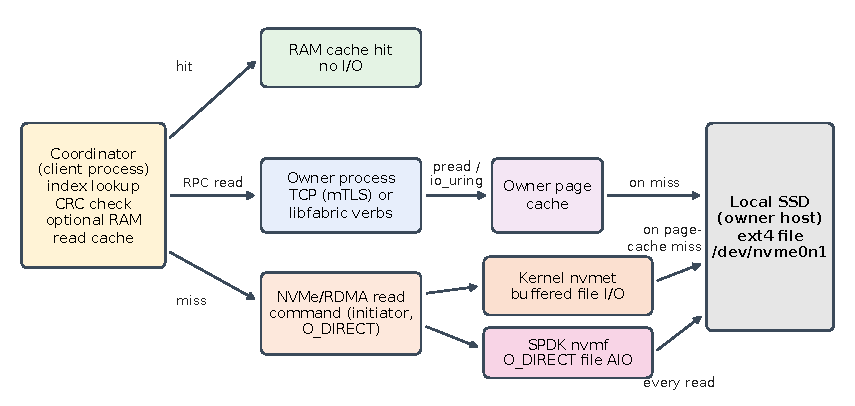
\includegraphics[width=.97\linewidth]{figures/readpaths.pdf}
\caption{Read routes. The coordinator holds the index and an optional RAM read cache. A miss goes to the owner process (TCP or verbs RPC) or becomes an NVMe/RDMA read command to the owner host. Writes send a whole batch to one owner, which acknowledges after a covering persistence barrier of its Value WAL.}\label{fig:paths}
\end{figure}
A cache hit does no I/O. On a miss, the TCP and verbs backends ask the owner process, which reads its Value WAL through the owner page cache. The NVMe-oF backends read the owner's WAL file over NVMe/RDMA instead. The kernel target reads through a buffered file and uses its page cache. The SPDK target uses \texttt{O\_DIRECT} file AIO and never uses the page cache. The sealed route reads immutable WAL files. The live route reads active WAL files. RF1 means one durable owner and no replication.

The queue geometry differs by route. The sealed initiator requested 4 I/O queues of depth 128 and observed 5 queues with \texttt{sqsize} 127 (case 0018, \path{nvme-host-0.json}). The live initiator requests 1 queue of depth 32 (\path{tidehunter/src/distributed/nvmeof/live_connect.rs:18-19}, also in the campaign package). The initiator opens the namespace with \texttt{O\_DIRECT} in both routes.

\section{Method and interpretation}\label{sec:method}
\textbf{Contracts.} Valkey puts use AOF \texttt{appendfsync=always} (observed). Tidehunter acknowledges after the owner's Value-WAL persistence barrier, including the Native baseline. The paper's default acknowledgement does not wait for fsync (Section 3.1 of \cite{tidehunter}); the stricter tier is used here to match Valkey. Garnet (AOF commit wait) and Kvrocks (RocksDB WAL, \texttt{sync=yes}) have observed fsync settings. Cassandra, FoundationDB and TiKV do not: their device fsync was not verified. Valkey GET reads RAM. Native Tidehunter has no network hop.
\textbf{Other stores.} Valkey, TiKV, Cassandra, FoundationDB, Kvrocks and Garnet were not run again. Each value is the median, over all GCP runs that completed the same population (store, transport, cohort, profile, value size, key count, concurrency, offered rate, operation and outcome), of that run's quantile: \N{S:ext_pops} populations with \N{S:ext_runs_min} to \N{S:ext_runs_max} runs each. The median of per-run quantiles is not a quantile of pooled calls. The runs come from different fleets and days, and not always from the same binaries. For one population, the p50 of the slowest run exceeds the p50 of the fastest run by a median factor of \N{S:ext_spread_med|.2f} (90th percentile \N{S:ext_spread_p90|.2f}, maximum \N{S:ext_spread_max|.2f}; \N{S:ext_spread_n} populations with at least two runs). A Tidehunter value is one run of the final fleet. A ratio between a Tidehunter value and the value of another store therefore carries at least this spread. Section~\ref{sec:drift} compares the unchanged stores between two campaigns and uses their final-run values, not medians.

\textbf{Quantiles.} API time is completion minus dispatch. Quantiles are exact nearest rank within one operation and outcome population (success only). Calls per second divide successful calls by the case duration, not by a steady-state interval. Rejected arrivals have no API latency and are counted apart. Statements marked \inference\ are reasoning, not measurements.

\textbf{Run noise.} The sealed read cases ran twice, once for each durability tier used to build the dataset: \N{S:twin_pairs} twin pairs. Their p50 ratios span \N{S:twin_p50_lo|.2f} to \N{S:twin_p50_hi|.2f} (median \N{S:twin_p50_med|.2f}). Their p99 ratios span \N{S:twin_p99_lo|.2f} to \N{S:twin_p99_hi|.2f}. This report treats p50 differences below 10 percent and p99 differences below a factor of two as run noise. The twins are two executions on one fleet, not independent repetitions.

\textbf{Device evidence.} Every case records block-device counters of all six hosts at the measurement gates. The Local SSD is \texttt{/dev/nvme0n1} on every host. \emph{Device reads per call} is the number of reads completed on the five owner hosts, divided by successful calls (the coordinator\textquoteright s own SSD for Native). The NVMe-oF initiator\textquoteright s namespaces give its command count and mean command time. These counters show whether a read reached an SSD. They do not show which read caused it.

\textbf{Limits.} Cold-OS cases have 4,096 calls and last \N{el:native:cold_os_cache:cold-os-large:read:65536} s (Native) to \N{el:th_spdk:cold_os_cache:cold-os-large:read:65536} s (SPDK). Throughput numbers are closed-loop at concurrency 16 or less. They are not saturation limits. All \N{S:cases_completed} completed cases are admitted, including twelve live SPDK cases that an earlier strict report rejected for a floating-point summation difference in one derived mean.

\section{Where Tidehunter is better and where it is not}
\begin{figure}[!htbp]\centering
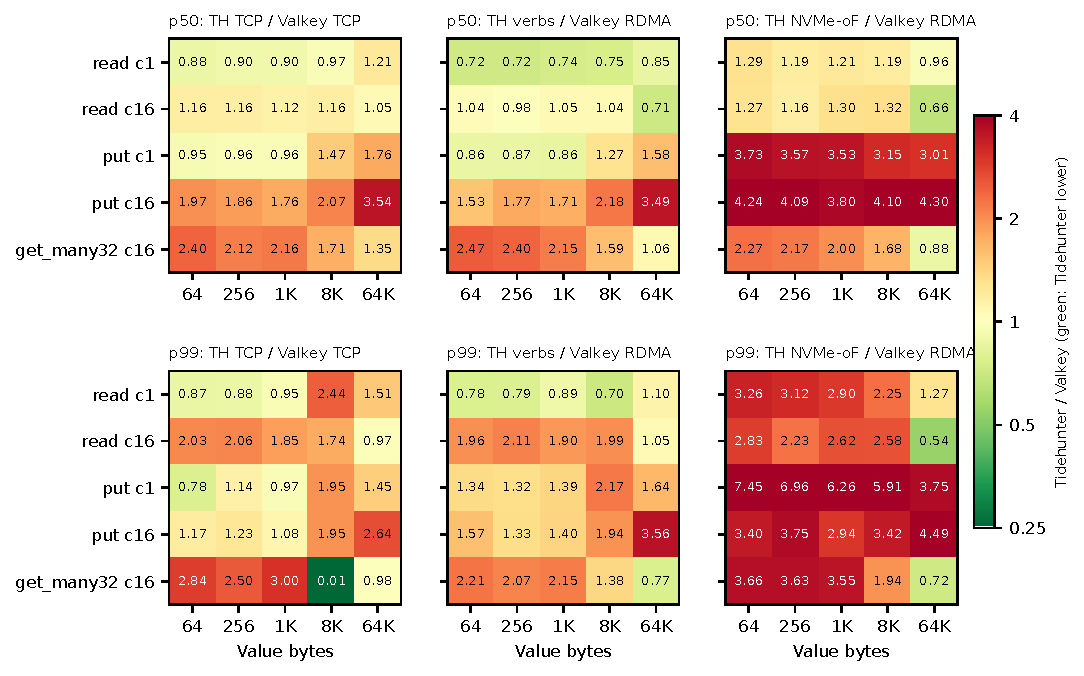
\includegraphics[width=.98\linewidth]{figures/scoreboard.pdf}
\caption{Tidehunter over Valkey: ratio of success-only API p50 (top) and p99 (bottom). Green means Tidehunter is lower. The c1 rows are the mixed point-operation profile; the others are the primary c16 cases. \runs. Valkey GET reads RAM and Valkey puts use AOF always; Tidehunter reads owner or target memory and puts persist with a covering fsync.}\label{fig:score}
\end{figure}
\begin{table}[!htbp]\centering
\small
\begin{tabular}{lrrr|rrr}\toprule
& \multicolumn{3}{c|}{Scalar read} & \multicolumn{3}{c}{Scalar write}\\
Backend & p50 & p99 & calls/s & p50 & p99 & calls/s\\\midrule
Native & 1.37 & 2.18 & 277{,}534 & 63.8 & 168 & 168{,}290\\
TH TCP & 60.1 & 209 & 172{,}074 & 322 & 506 & 47{,}427\\
TH verbs & 45.0 & 176 & 220{,}750 & 295 & 575 & 51{,}467\\
TH NVMe-oF kernel & 55.9 & 242 & 181{,}799 & 657 & 1{,}206 & 23{,}841\\
TH NVMe-oF SPDK & 71.7 & 156 & 147{,}290 & 702 & 1{,}248 & 22{,}172\\
Valkey TCP & 53.4 & 113 & 188{,}256 & 183 & 469 & 73{,}443\\
Valkey RDMA & 43.1 & 92.5 & 165{,}026 & 173 & 410 & 80{,}146\\
\bottomrule\end{tabular}

\caption{1 KiB scalar calls at concurrency 16: success-only API p50 and p99 in \us, and successful calls/s. \runs.}\label{tab:onekib1}
\end{table}
\begin{table}[!htbp]\centering
\small
\begin{tabular}{lrrr|rrr}\toprule
& \multicolumn{3}{c|}{Read-many32} & \multicolumn{3}{c}{Write-batch32}\\
Backend & p50 & p99 & calls/s & p50 & p99 & calls/s\\\midrule
Native & 55.3 & 113 & 110{,}340 & 1{,}047 & 1{,}247 & 13{,}901\\
TH TCP & 840 & 2{,}418 & 16{,}895 & 2{,}554 & 3{,}576 & 6{,}363\\
TH verbs & 688 & 1{,}723 & 19{,}913 & 2{,}256 & 3{,}212 & 7{,}191\\
TH NVMe-oF kernel & 641 & 2{,}846 & 18{,}272 & 2{,}421 & 3{,}810 & 6{,}322\\
TH NVMe-oF SPDK & 642 & 2{,}740 & 18{,}391 & 2{,}253 & 4{,}030 & 6{,}405\\
Valkey TCP & 389 & 807 & 29{,}860 & -- & -- & --\\
Valkey RDMA & 321 & 803 & 35{,}821 & -- & -- & --\\
\bottomrule\end{tabular}

\caption{1 KiB 32-key calls at concurrency 16. Valkey has no batch-write case; a dash is not zero.}\label{tab:onekib2}
\end{table}
\textbf{Better.}
\begin{itemize}
\item \emph{Concurrency-1 reads.} Verbs over Valkey RDMA has p50 ratios of \N{ratio:p50:th_verbs/valkey_rdma:primary_rf1:point-mixed:read:256} to \N{ratio:p50:th_verbs/valkey_rdma:primary_rf1:point-mixed:read:8192} for 64~B to 8~KiB and \N{ratio:p50:th_verbs/valkey_rdma:primary_rf1:point-mixed:read:65536} at 64~KiB. TCP over Valkey TCP has \N{ratio:p50:th_tcp/valkey_tcp:primary_rf1:point-mixed:read:64} to \N{ratio:p50:th_tcp/valkey_tcp:primary_rf1:point-mixed:read:8192} up to 8~KiB and \N{ratio:p50:th_tcp/valkey_tcp:primary_rf1:point-mixed:read:65536} at 64~KiB.
\item \emph{Concurrency-1 puts up to 1~KiB.} Verbs over Valkey RDMA has p50 ratios of \N{ratio:p50:th_verbs/valkey_rdma:primary_rf1:point-mixed:put:64}, \N{ratio:p50:th_verbs/valkey_rdma:primary_rf1:point-mixed:put:256} and \N{ratio:p50:th_verbs/valkey_rdma:primary_rf1:point-mixed:put:1024}. Valkey is faster from 8~KiB (\N{ratio:p50:th_verbs/valkey_rdma:primary_rf1:point-mixed:put:8192} and \N{ratio:p50:th_verbs/valkey_rdma:primary_rf1:point-mixed:put:65536}). The p99 ratios are above 1 (\N{ratio:p99:th_verbs/valkey_rdma:primary_rf1:point-mixed:put:64} to \N{ratio:p99:th_verbs/valkey_rdma:primary_rf1:point-mixed:put:1024}).
\item \emph{Large values at concurrency 16.} For 64~KiB reads, verbs has p50 \N{ratio:p50:th_verbs/valkey_rdma:primary_rf1:read-concurrent:read:65536}$\times$ and throughput \N{xratio:cps:th_verbs:primary_rf1:read-concurrent:valkey_rdma:primary_rf1:read-concurrent:read:65536}$\times$ that of Valkey RDMA (\RC{gibs}{th_verbs}{65536} against \RC{gibs}{valkey_rdma}{65536}~GiB/s). The kernel target has p50 \N{ratio:p50:th_kernel/valkey_rdma:primary_rf1:read-concurrent:read:65536}$\times$ and p99 \N{ratio:p99:th_kernel/valkey_rdma:primary_rf1:read-concurrent:read:65536}$\times$. For 32-key reads of 64~KiB the kernel target has p50 \N{ratio:p50:th_kernel/valkey_rdma:primary_rf1:read-many32:get_many:65536}$\times$.
\item \emph{Cache hits.} A coordinator-cache hit has p50 \CC{p50}{th_verbs}{256} to \CC{p50}{th_tcp}{8192}~\us, against \PR{p50}{valkey_rdma}{256} to \PR{p50}{valkey_rdma}{8192}~\us\ for a Valkey RDMA read at concurrency 1.
\item \emph{Other stores.} At 1~KiB, verbs and TCP have a lower p50 than all five other stores for c1 reads (\PR{p50}{th_verbs}{1024} and \PR{p50}{th_tcp}{1024}~\us, against \PR{p50}{kvrocks}{1024} for Kvrocks, the best of the five), c16 reads (\RC{p50}{th_verbs}{1024} and \RC{p50}{th_tcp}{1024}~\us, against \RC{p50}{garnet}{1024} for Garnet) and 32-key reads (\MR{p50}{th_verbs}{1024} and \MR{p50}{th_tcp}{1024}~\us, against \MR{p50}{cassandra}{1024} for Cassandra).
\end{itemize}
\textbf{Not better.}
\begin{itemize}
\item \emph{Puts at concurrency 16.} Verbs over Valkey RDMA has p50 ratios of \N{ratio:p50:th_verbs/valkey_rdma:primary_rf1:write-concurrent:put:64} to \N{ratio:p50:th_verbs/valkey_rdma:primary_rf1:write-concurrent:put:8192} for 64~B to 8~KiB and \N{ratio:p50:th_verbs/valkey_rdma:primary_rf1:write-concurrent:put:65536} at 64~KiB. At 1~KiB the calls/s are \WC{cps}{th_verbs}{1024} against \WC{cps}{valkey_rdma}{1024}. The live NVMe-oF puts are \N{ratio:p50:th_kernel/valkey_rdma:primary_rf1:write-concurrent:put:1024}$\times$ (kernel) and \N{ratio:p50:th_spdk/valkey_rdma:primary_rf1:write-concurrent:put:1024}$\times$ (SPDK) Valkey RDMA at 1~KiB.
\item \emph{Scaling with concurrency.} From c1 to c16 at 1~KiB, the verbs put p50 grows \N{xratio:p50:th_verbs:primary_rf1:write-concurrent:th_verbs:primary_rf1:point-mixed:put:1024}$\times$ (\PP{p50}{th_verbs}{1024} to \WC{p50}{th_verbs}{1024}~\us) and the Valkey RDMA put p50 grows \N{xratio:p50:valkey_rdma:primary_rf1:write-concurrent:valkey_rdma:primary_rf1:point-mixed:put:1024}$\times$ (\PP{p50}{valkey_rdma}{1024} to \WC{p50}{valkey_rdma}{1024}~\us). Verbs puts beat Valkey at c1 and lose at c16. The read p50 grows \N{xratio:p50:th_verbs:primary_rf1:read-concurrent:th_verbs:primary_rf1:point-mixed:read:1024}$\times$ for verbs and \N{xratio:p50:valkey_rdma:primary_rf1:read-concurrent:valkey_rdma:primary_rf1:point-mixed:read:1024}$\times$ for Valkey RDMA.
\item \emph{32-key reads.} Verbs over Valkey RDMA has p50 ratios of \N{ratio:p50:th_verbs/valkey_rdma:primary_rf1:read-many32:get_many:256} to \N{ratio:p50:th_verbs/valkey_rdma:primary_rf1:read-many32:get_many:64} up to 1~KiB and \N{ratio:p50:th_verbs/valkey_rdma:primary_rf1:read-many32:get_many:8192} at 8~KiB. At 1~KiB that is \N{p50:th_verbs:primary_rf1:read-many32:get_many:1024|.0f}~\us\ against \N{p50:valkey_rdma:primary_rf1:read-many32:get_many:1024|.0f}~\us\ per call of 32 keys.
\item \emph{Read tails at concurrency 16.} Verbs p99 over Valkey RDMA p99 is \N{ratio:p99:th_verbs/valkey_rdma:primary_rf1:read-concurrent:read:8192} to \N{ratio:p99:th_verbs/valkey_rdma:primary_rf1:read-concurrent:read:64} up to 8~KiB. TCP over Valkey TCP is \N{ratio:p99:th_tcp/valkey_tcp:primary_rf1:read-concurrent:read:8192} to \N{ratio:p99:th_tcp/valkey_tcp:primary_rf1:read-concurrent:read:64}. At 64~KiB the verbs ratio is \N{ratio:p99:th_verbs/valkey_rdma:primary_rf1:read-concurrent:read:65536} and the kernel-target ratio is \N{ratio:p99:th_kernel/valkey_rdma:primary_rf1:read-concurrent:read:65536}.
\item \emph{NVMe-oF reads of small values.} At concurrency 1 and 1~KiB, the mixed-profile read p50 is \PR{p50}{th_kernel}{1024}~\us\ (kernel target) and \PR{p50}{th_spdk}{1024}~\us\ (SPDK target), against \PR{p50}{th_verbs}{1024}~\us\ for the verbs owner RPC.
\end{itemize}

\section{Workload curves}
Figure~\ref{fig:primary} gives the primary RF1 curves and Figure~\ref{fig:point} the concurrency-1 mixed point operations. Section~\ref{sec:others} compares the other stores.
\begin{figure}[!htbp]\centering
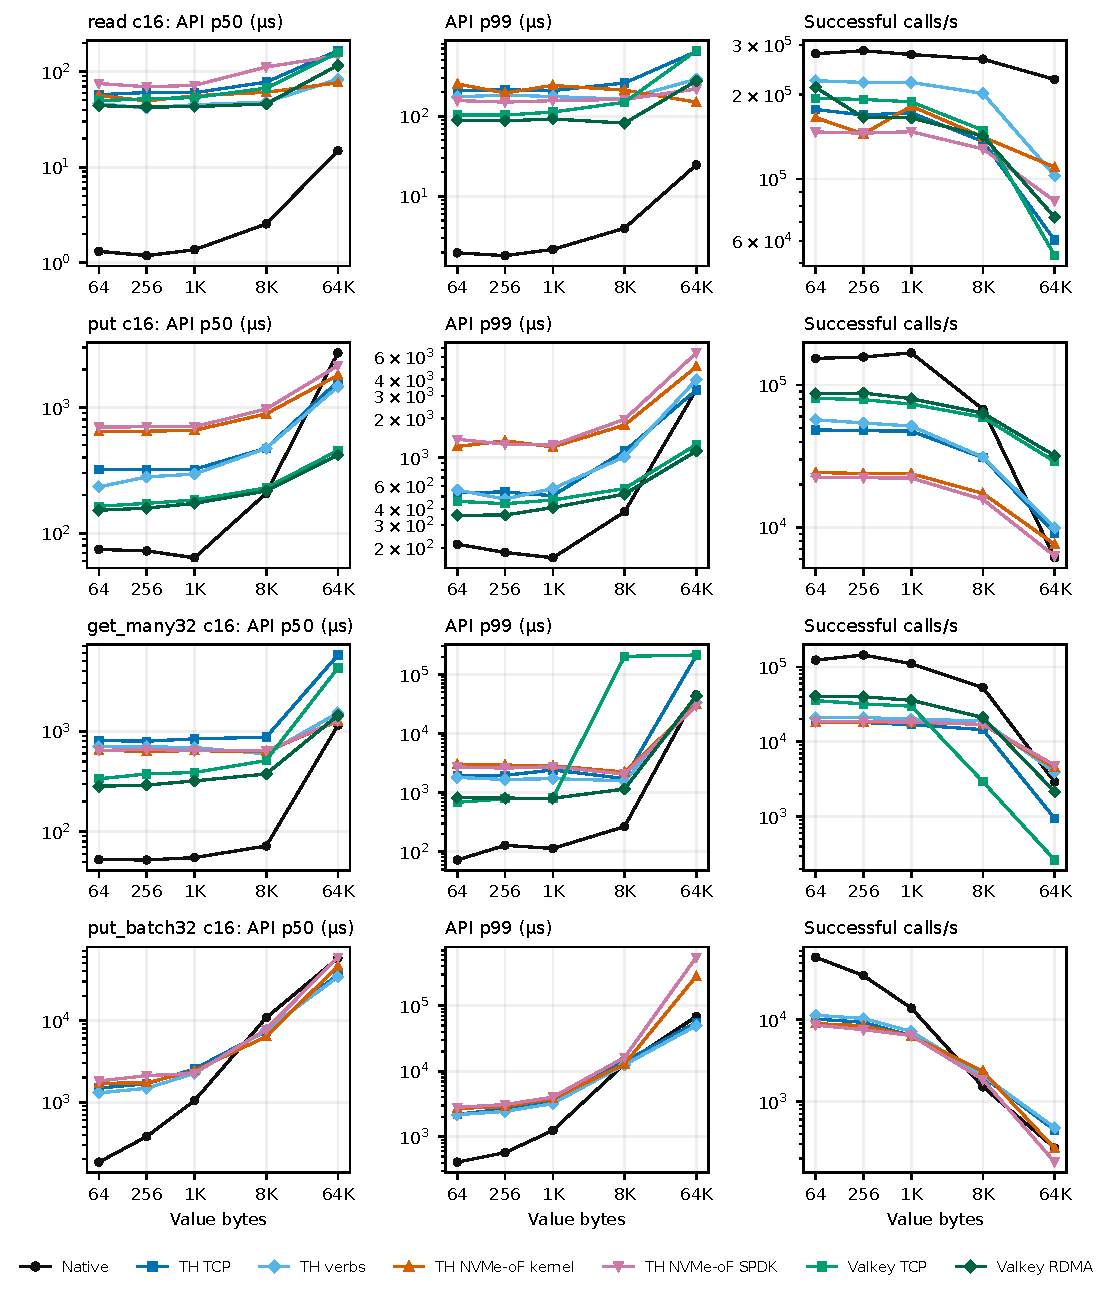
\includegraphics[width=.98\linewidth]{figures/primary.pdf}
\caption{RF1 calls at concurrency 16: scalar reads (8,192 calls per case), scalar puts (4,096), 32-key reads and 32-key writes (2,048 calls per case; one call covers 32 values). API p50, API p99 and successful calls/s against value size. \runs. Valkey has no batch-write case. Valkey TCP 32-key p99 includes stalls of \MR{p99ms}{valkey_tcp}{8192}~ms at 8~KiB and \MR{p99ms}{valkey_tcp}{65536}~ms at 64~KiB. Hollow SPDK markers: API latency kept, target counters not admitted. The Tidehunter coordinator cache is disabled. Owner and kernel-target page caches serve these reads (Table~\ref{tab:media}); the SPDK path reads the SSD. Valkey GET reads RAM.}\label{fig:primary}
\end{figure}
\begin{figure}[!htbp]\centering
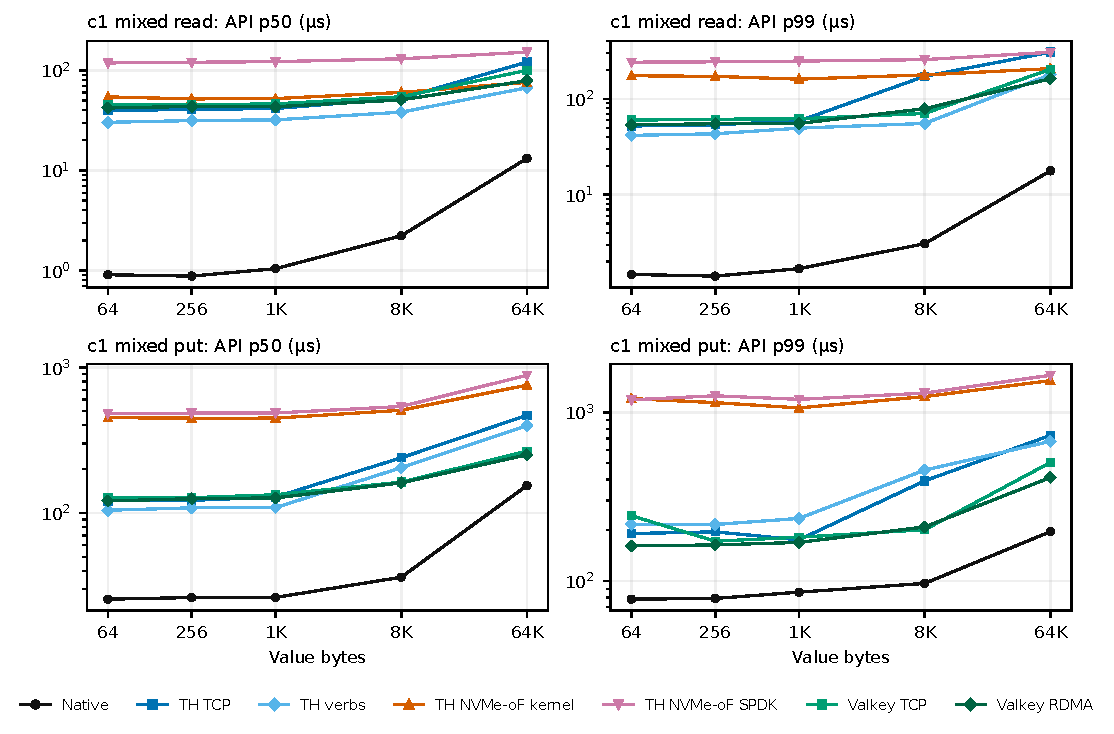
\includegraphics[width=.98\linewidth]{figures/point.pdf}
\caption{Concurrency-1 mixed point operations: API p50 and p99 of reads and puts that run interleaved. \runs. SPDK reads include an SSD read on every call (Table~\ref{tab:media}).}\label{fig:point}
\end{figure}

\section{Other stores}\label{sec:others}
\begin{figure}[!htbp]\centering
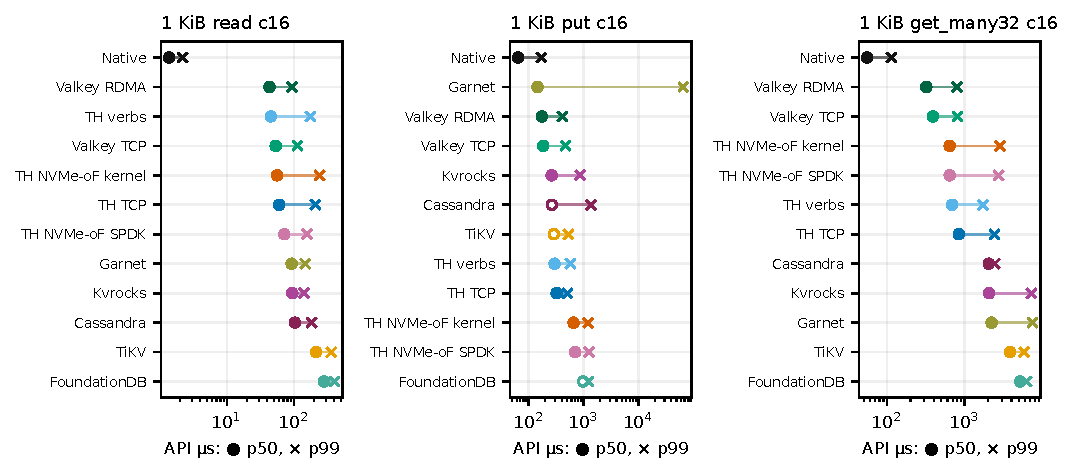
\includegraphics[width=.98\linewidth]{figures/others.pdf}
\caption{All stores at 1~KiB, concurrency 16: API p50 (dot) and p99 (cross), sorted by p50. In the put panel a hollow dot marks a store whose device fsync was not verified (Cassandra, FoundationDB, TiKV).}\label{fig:others}
\end{figure}
Table~\ref{tab:stores} gives the values. Tidehunter reads and 32-key reads are faster than all five other stores. Tidehunter puts are not: Cassandra (\WC{p50}{cassandra}{1024}~\us), Kvrocks (\WC{p50}{kvrocks}{1024}), TiKV (\WC{p50}{tikv}{1024}) and Garnet (\WC{p50}{garnet}{1024}; its p99 is \WC{p99ms}{garnet}{1024}~ms) are below verbs (\WC{p50}{th_verbs}{1024}) and TCP (\WC{p50}{th_tcp}{1024}). FoundationDB is above both (\WC{p50}{foundationdb}{1024}). At 50,000 offered operations per second, Garnet rejects \N{rej:garnet:50000} of 400,000 calls (Section~\ref{sec:offered}).
\begin{table}[!htbp]\centering
\small
\begin{tabular}{lrrrrr}\toprule
Store & read c1 & read c16 & put c1 & put c16 & get\_many32 c16\\\midrule
Native & 1.04/1.68 & 1.37/2.18 & 26.3/86.0 & 63.8/168 & 55.3/113\\
TH TCP & 41.5/58.7 & 60.1/209 & 129/176 & 322/506 & 840/2{,}418\\
TH verbs & 32.0/49.4 & 45.0/176 & 109/235 & 295/575 & 688/1{,}723\\
TH NVMe-oF kernel & 52.2/161 & 55.9/242 & 448/1{,}061 & 657/1{,}206 & 641/2{,}846\\
TH NVMe-oF SPDK & 122/248 & 71.7/156 & 486/1{,}193 & 702/1{,}248 & 642/2{,}740\\
Valkey TCP & 46.2/61.9 & 53.4/113 & 133/182 & 183/469 & 389/807\\
Valkey RDMA & 43.2/55.3 & 43.1/92.5 & 127/170 & 173/410 & 321/803\\
TiKV & 91.0/122 & 214/362 & 169/280 & 286/527 & 3{,}840/5{,}871\\
Cassandra & 139/220 & 104/184 & 203/448 & 263/1{,}362 & 2{,}043/2{,}446\\
FoundationDB & 480/4{,}786 & 281/402 & 915/1{,}070 & 986/1{,}233 & 5{,}203/6{,}321\\
Kvrocks & 50.0/62.1 & 94.4/141 & 135/166 & 262/864 & 2{,}061/7{,}242\\
Garnet & 58.7/72.6 & 92.2/147 & 101/164 & 144/66{,}736 & 2{,}221/7{,}475\\
\bottomrule\end{tabular}

\caption{All stores at 1~KiB: API p50/p99 in \us. c1 cells are the mixed point-operation profile. \runs. Acknowledgement contracts differ (Section 3).}\label{tab:stores}
\end{table}

\section{Remote NVMe reads}\label{sec:nvme}
\subsection{What the owner disk saw}
Latency alone does not show whether a read reached an SSD. Table~\ref{tab:media} gives block-device reads per call.
\begin{table}[!htbp]\centering
\small
\begin{tabular}{l|rrrrr|r|rr|r}\toprule
& \multicolumn{5}{c|}{First-touch c1, value bytes} & Repeat c1 & \multicolumn{2}{c|}{Live read c16} & Cold c16\\
Path & 64 & 256 & 1K & 8K & 64K & 64K & 1K & 64K & 64K\\\midrule
Native & 0.004 & 0.004 & 0.017 & 0.073 & 0.512 & 0.000 & 0.000 & 0.000 & 0.782\\
TH TCP & 0.006 & 0.011 & 0.025 & 0.094 & 0.542 & 0.000 & 0.000 & 0.000 & 4.182\\
TH verbs & 0.029 & 0.075 & 0.263 & 1.001 & 1.001 & 0.000 & 0.000 & 0.000 & 4.151\\
Kernel NVMe-oF & 0.006 & 0.011 & 0.025 & 0.094 & 1.008 & 0.000 & 0.000 & 0.000 & 1.110\\
SPDK NVMe-oF & 1.011 & 1.013 & 1.043 & 1.045 & 1.013 & 1.000 & 1.009 & 1.009 & 1.185\\
\bottomrule\end{tabular}

\caption{Block-device reads per call on the owner hosts (the coordinator\textquoteright s SSD for Native), from \texttt{/proc/diskstats} at the measurement gates. Zero means every read came from memory. One means a device read for each call. Live reads cover data written during the run.}\label{tab:media}
\end{table}
Four results follow. (1) In the repeat pass the TCP, verbs and kernel paths read no SSD. The SPDK path reads the SSD on every call (\RR{dev}{th_spdk}{65536}), because its target bypasses the page cache. (2) After a cache drop, a first-touch key sweep still hits memory for most small reads: the kernel target and the TCP owner issue \FT{dev}{th_kernel}{64} to \FT{dev}{th_kernel}{8192} device reads per call up to 8~KiB. (3) The verbs owner reads the SSD on every call from 8~KiB (\FT{dev}{th_verbs}{8192}) and the TCP owner does not (\FT{dev}{th_tcp}{8192}). First-touch cases of these two paths do not compare the transports (Section~\ref{sec:coherence}). (4) Only SPDK (all sizes), verbs (8~KiB and above) and the kernel target at 64~KiB (\FT{dev}{th_kernel}{65536}) read the SSD on every first-touch call. At cold 64~KiB, every path that stores its data on the SSD reads it (Figure~\ref{fig:cold}).

\subsection{Cost of one remote read at concurrency 1}
Table~\ref{tab:readcost} compares the paths in the repeat pass, where every path except SPDK reads memory. Table~\ref{tab:nvmecmd} adds the device evidence of the first-touch pass.
\begin{table}[!htbp]\centering
\small
\begin{tabular}{lrrrrr}\toprule
Path, p50 / p99 \us & 64 B & 256 B & 1 KiB & 8 KiB & 64 KiB\\\midrule
Native (local) & 0.70/1.14 & 0.70/1.15 & 1.07/1.56 & 2.54/3.41 & 11.6/17.5\\
Owner RPC, TCP & 40.1/49.0 & 39.4/49.6 & 41.1/51.4 & 55.1/67.7 & 99.5/118\\
Owner RPC, verbs & 31.6/39.6 & 32.1/42.0 & 33.4/43.2 & 39.4/48.1 & 59.8/71.7\\
NVMe-oF, kernel target & 39.6/48.4 & 37.9/46.2 & 39.4/47.4 & 45.1/53.8 & 61.0/73.7\\
NVMe-oF, SPDK target & 59.2/70.3 & 58.7/71.1 & 97.8/124 & 120/136 & 133/148\\
\bottomrule\end{tabular}

\caption{Sealed repeat-pass scalar reads at concurrency 1 (8,192 calls per case): API p50/p99 in \us. Native, the owner RPC and the kernel target read memory. The SPDK target reads its SSD on every call (Table~\ref{tab:media}). One repetition.}\label{tab:readcost}
\end{table}
\begin{table}[!htbp]\centering
\scriptsize
\resizebox{\linewidth}{!}{%
\begin{tabular}{rrr|rrrr|rrrrr}\toprule
& \multicolumn{2}{c|}{Initiator} & \multicolumn{4}{c|}{Kernel target (buffered file)} & \multicolumn{5}{c}{SPDK target (O\_DIRECT file AIO)}\\
Value B & B/call & $\times$ & p50 & p99 & cmd \us & dev/call & p50 & p99 & cmd \us & dev/call & dev \us\\\midrule
64 & 4{,}192 & 65.5 & 36.1 & 50.7 & 24.2 & 0.006 & 54.3 & 70.1 & 40.9 & 1.011 & 25.0\\
256 & 4{,}384 & 17.1 & 35.0 & 45.5 & 23.2 & 0.011 & 55.2 & 75.4 & 41.5 & 1.013 & 24.8\\
1{,}024 & 5{,}152 & 5.0 & 36.5 & 56.9 & 23.8 & 0.025 & 59.2 & 128 & 48.7 & 1.043 & 43.2\\
8{,}192 & 12{,}322 & 1.5 & 40.2 & 154 & 26.1 & 0.094 & 99.7 & 222 & 79.5 & 1.045 & 68.1\\
65{,}536 & 69{,}632 & 1.1 & 54.3 & 357 & 53.0 & 1.008 & 132 & 257 & 113.6 & 1.013 & 87.2\\
\bottomrule\end{tabular}}

\caption{Sealed first-touch scalar reads at concurrency 1 ($n=8{,}192$ per case). p50 and p99 are API latencies in \us. B/call is the initiator\textquoteright s read volume per call and $\times$ its ratio to the value size. cmd is the mean block-layer time of one NVMe read at the initiator. dev/call is device reads per call on the owner hosts and dev the mean block-layer time of one such read.}\label{tab:nvmecmd}
\end{table}

\textbf{Without media.} The kernel target answers from page cache. The initiator command takes \FT{initus}{th_kernel}{256} to \FT{initus}{th_kernel}{8192}~\us\ up to 8~KiB, and the API p50 is \FT{p50}{th_kernel}{256} to \FT{p50}{th_kernel}{8192}~\us. Client work adds \N{clientus:th_kernel:sealed_read:first_touch-scalar-c1-baseline:read:256} to \N{clientus:th_kernel:sealed_read:first_touch-scalar-c1-baseline:read:8192}~\us\ (mean API time minus mean command time). The owner RPC costs \RR{p50}{th_verbs}{64} to \RR{p50}{th_verbs}{1024}~\us\ over verbs and \RR{p50}{th_tcp}{256} to \RR{p50}{th_tcp}{1024}~\us\ over TCP in the repeat pass. A local first-touch read costs \FT{p50}{native}{256} to \FT{p50}{native}{8192}~\us. A remote read therefore costs about as much as an owner RPC, and \N{ratio:p50:th_kernel/native:sealed_read:first_touch-scalar-c1-baseline:read:8192|.0f} to \N{ratio:p50:th_kernel/native:sealed_read:first_touch-scalar-c1-baseline:read:256|.0f} times a local first-touch read.

\textbf{With media on every call.} The SPDK initiator command takes \FT{initus}{th_spdk}{64}~\us\ for a 4~KiB read, of which the target SSD read takes \FT{devus}{th_spdk}{64}~\us. The other \N{S:spdk_fabric_us|.0f}~\us\ is fabric and target software. API p50 is \FT{p50}{th_spdk}{64} to \FT{p50}{th_spdk}{1024}~\us\ up to 1~KiB, \FT{p50}{th_spdk}{8192}~\us\ at 8~KiB and \FT{p50}{th_spdk}{65536}~\us\ at 64~KiB. The SSD read time per device read grows from \FT{devus}{th_spdk}{64}~\us\ to \FT{devus}{th_spdk}{65536}~\us.

\textbf{Read amplification.} The initiator reads aligned 4~KiB blocks, one NVMe read per call: \N{amp:th_kernel:sealed_read:first_touch-scalar-c1-baseline:read:64}$\times$ the value size at 64~B, \N{amp:th_kernel:sealed_read:first_touch-scalar-c1-baseline:read:256}$\times$ at 256~B, \N{amp:th_kernel:sealed_read:first_touch-scalar-c1-baseline:read:1024}$\times$ at 1~KiB, \N{amp:th_kernel:sealed_read:first_touch-scalar-c1-baseline:read:8192}$\times$ at 8~KiB and \N{amp:th_kernel:sealed_read:first_touch-scalar-c1-baseline:read:65536}$\times$ at 64~KiB. On a page-cache hit this wastes fabric bytes only. On the SPDK path it wastes SSD bandwidth.

\begin{figure}[!htbp]\centering
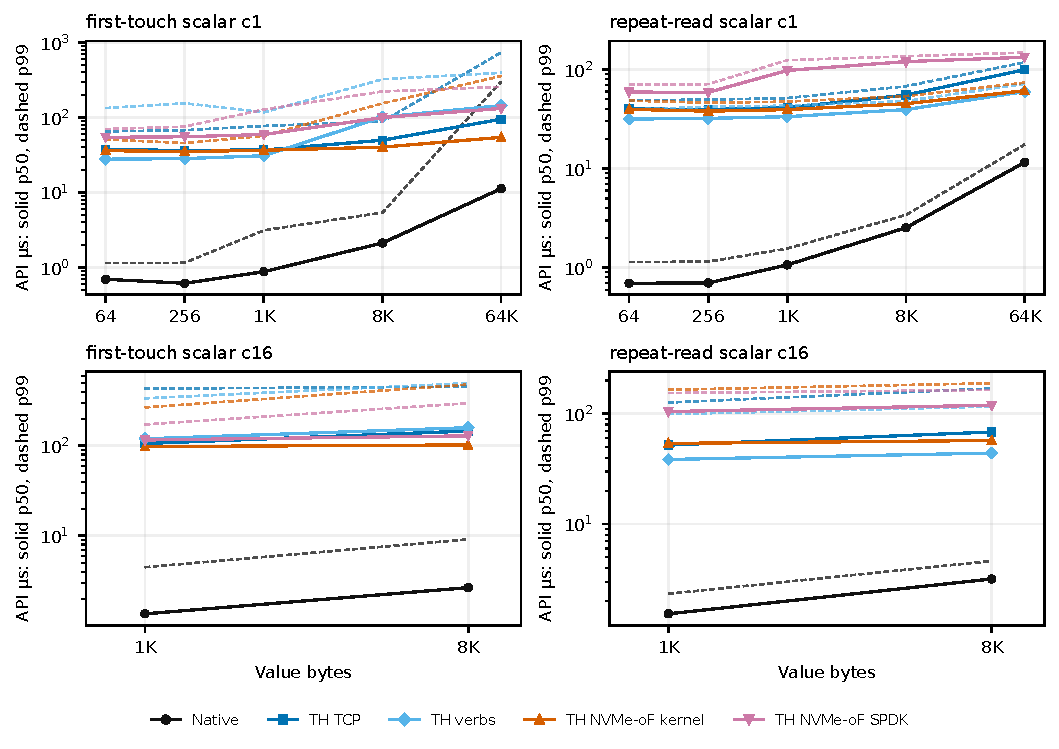
\includegraphics[width=.98\linewidth]{figures/sealed.pdf}
\caption{Sealed scalar reads, first-touch (cache drop and key sweep) and repeat, at concurrency 1 and 16 (8,192 calls per case): API p50 (solid) and p99 (dashed). One repetition. The media state differs between paths (Table~\ref{tab:media}), so the transports are not compared here. Native is local.}\label{fig:sealed}
\end{figure}

\subsection{Cold reads of a large dataset}
\begin{figure}[!htbp]\centering
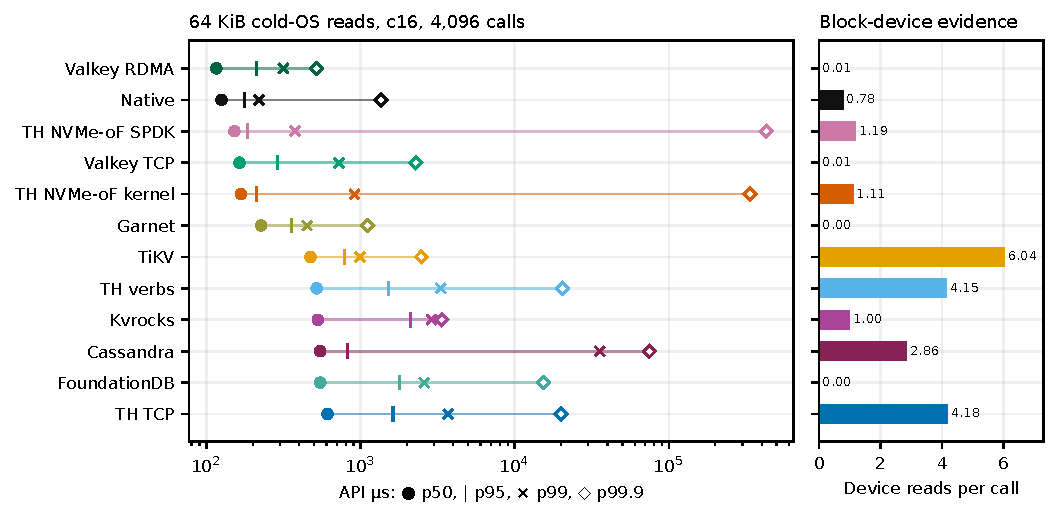
\includegraphics[width=.98\linewidth]{figures/cold.pdf}
\caption{64~KiB reads of 131,072 keys (8~GiB) after a cache drop, concurrency 16, 4,096 calls per case. Left: API p50, p95, p99 and p99.9 (\runs). Right: device reads per call in the final run. Valkey, FoundationDB and Garnet serve the data from memory, so their cold numbers are not SSD numbers.}\label{fig:cold}
\end{figure}
In this cohort every Tidehunter path reads the SSD. Local Tidehunter has p50 \CO{p50}{native}{65536}~\us\ and p99 \CO{p99}{native}{65536}~\us. The kernel target has \CO{p50}{th_kernel}{65536} and \CO{p99}{th_kernel}{65536}~\us, and the SPDK target \CO{p50}{th_spdk}{65536} and \CO{p99}{th_spdk}{65536}~\us. A remote read therefore adds \N{more:p50:th_spdk/native:cold_os_cache:cold-os-large:read:65536} to \N{more:p50:th_kernel/native:cold_os_cache:cold-os-large:read:65536} percent to the local p50.

The owner RPC is slower: p50 is \CO{p50}{th_verbs}{65536}~\us\ (verbs) and \CO{p50}{th_tcp}{65536}~\us\ (TCP), \N{ratio:p50:th_verbs/th_kernel:cold_os_cache:cold-os-large:read:65536} to \N{ratio:p50:th_tcp/th_spdk:cold_os_cache:cold-os-large:read:65536} times the NVMe-oF p50. The owner issues \N{dev:th_tcp:cold_os_cache:cold-os-large:read:65536|.1f} device reads per call and NVMe-oF issues \N{dev:th_kernel:cold_os_cache:cold-os-large:read:65536|.1f} to \N{dev:th_spdk:cold_os_cache:cold-os-large:read:65536|.1f}. The code submits one \texttt{io\_uring} read per value member (\path{distributed/tcp/read_executor.rs:828-836}), so the mechanism that splits the read is not determined (Section~\ref{sec:next}).

The cold NVMe-oF cases contain one stall each: p99.9 is \N{p999ms:th_kernel:cold_os_cache:cold-os-large:read:65536}~ms (kernel) and \N{p999ms:th_spdk:cold_os_cache:cold-os-large:read:65536}~ms (SPDK), in cases that last \N{el:th_kernel:cold_os_cache:cold-os-large:read:65536} and \N{el:th_spdk:cold_os_cache:cold-os-large:read:65536}~s. The stall dominates their mean (\CO{mean}{th_kernel}{65536} and \CO{mean}{th_spdk}{65536}~\us) and their calls/s (\CO{cps}{th_kernel}{65536} and \CO{cps}{th_spdk}{65536}). The owner RPC reaches \CO{cps}{th_tcp}{65536} to \CO{cps}{th_verbs}{65536} calls/s. The p50 and p99 above exclude the stall. Its cause is not determined.

\subsection{Throughput and policy}
At concurrency 16, live 64~KiB reads move \RC{gibs}{th_kernel}{65536}~GiB/s (kernel target, page cache), \RC{gibs}{th_spdk}{65536}~GiB/s (SPDK, SSD) and \RC{gibs}{th_verbs}{65536}~GiB/s (verbs RPC). Valkey RDMA moves \RC{gibs}{valkey_rdma}{65536}~GiB/s. These are closed-loop numbers of one client process. Peak NVMe-oF IOPS and bandwidth, NVMe/TCP and queue-depth sweeps were not measured.

\textbf{Where NVMe reads win.} Large values that miss RAM, measured at 64~KiB and c16 (Figure~\ref{fig:cold}): p50 is \N{ratio:p50:th_tcp/th_kernel:cold_os_cache:cold-os-large:read:65536}$\times$ lower and p99 is \N{ratio:p99:th_tcp/th_kernel:cold_os_cache:cold-os-large:read:65536}$\times$ lower than for the TCP owner. No media-matched comparison exists at 8~KiB.

\textbf{Where they lose or tie.} Small values. The owner RPC over verbs costs \RR{p50}{th_verbs}{64} to \RR{p50}{th_verbs}{1024}~\us\ against \FT{p50}{th_kernel}{256} to \FT{p50}{th_kernel}{1024}~\us\ for a page-cache NVMe read, and a 64~B value needs a 4~KiB read. Writes through the live NVMe-oF route cost \WC{p50}{th_kernel}{1024}~\us\ against \WC{p50}{th_verbs}{1024}~\us\ for the owner RPC.

\textbf{Policy} \inference. Try the coordinator cache first. Send small misses (up to about 1~KiB) to the owner RPC over verbs. Send large misses to NVMe-oF. Test the SPDK target where a read must reach the SSD: in the matched cold case its p99 was \N{ratio:p99:th_kernel/th_spdk:cold_os_cache:cold-os-large:read:65536}$\times$ lower, but its p50 difference of \N{lower:p50:th_spdk/th_kernel:cold_os_cache:cold-os-large:read:65536} percent is inside run noise and there is one run. Keep writes on the owner RPC.

\section{Cache, offered load and run-to-run}\label{sec:offered}\label{sec:drift}
\begin{figure}[!htbp]\centering
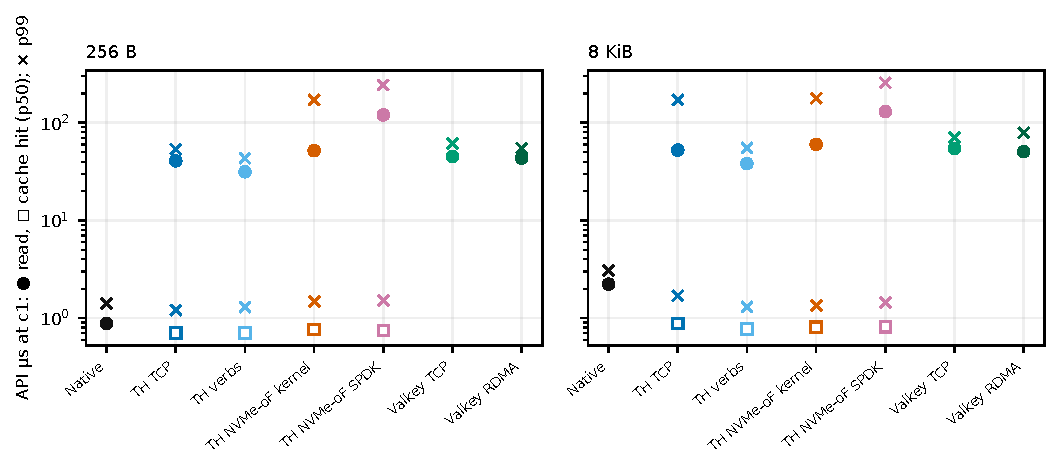
\includegraphics[width=.92\linewidth]{figures/cache.pdf}
\caption{Coordinator-cache hits (hollow squares, 128~MiB cache) against remote reads (circles) at concurrency 1: API p50 and p99 (\runs). The remote reads are the mixed point-operation reads. Valkey and Native have no cache cohort.}\label{fig:cache}
\end{figure}
A hit costs \CC{p50}{th_verbs}{256} to \CC{p50}{th_tcp}{8192}~\us. It is \N{S:hit_speedup_min|.0f} to \N{S:hit_speedup_max|.0f} times faster than a remote read at concurrency 1 on the same backend and size, and it uses neither the network nor a disk. In the binary of this campaign the cache is limited by entries as well as bytes: each slot is charged at least 1~KiB (\path{read_cache.rs:78,83,422-425}). A 128~MiB budget therefore holds fewer than 131,072 entries whatever the value size. A dataset of 64~B or 256~B values fills at most 6 or 25 percent of the budget with payload. After the campaign this accounting was replaced by an exact per-entry charge (\path{docs/distributed/FOCUSED_CAMPAIGN_2026-11-07.md}; synthetic and captured-trace evaluation in \path{fixes/cache-mrc-exact-accounting/} of the analysis directory). The numbers in this section describe the old accounting.
\begin{table}[!htbp]\centering
\small
\begin{tabular}{lr|rrrr}\toprule
Miss path & p50 \us\ & \multicolumn{4}{c}{hit ratio for a mean latency of}\\
 & & 20 \us & 10 \us & 5 \us & 2 \us\\\midrule
Owner RPC over verbs, c1 read, 1 KiB & 32.0 & 38.5\% & 70.5\% & 86.5\% & 96.2\%\\
Owner RPC over TCP, c1 read, 1 KiB & 41.5 & 52.8\% & 77.4\% & 89.7\% & 97.1\%\\
Kernel NVMe-oF (page cache), c1 read, 1 KiB & 52.2 & 62.6\% & 82.1\% & 91.8\% & 97.7\%\\
Kernel NVMe-oF, cold 64 KiB, c16 & 167 & 88.5\% & 94.5\% & 97.5\% & 99.3\%\\
Owner RPC over TCP, cold 64 KiB, c16 & 610 & 96.8\% & 98.5\% & 99.3\% & 99.8\%\\
\bottomrule\end{tabular}

\caption{Hit ratio $h=(L-g)/(L-H)$ that the coordinator cache needs for a mean read latency $g$. $L$ is the measured p50 of the miss path and $H=0.8$~\us\ the measured hit p50. This is an estimate from medians. Miss tails raise the real mean, so the ratios are lower bounds.}\label{tab:hit}
\end{table}
For a mean of 5~\us\ the 1~KiB miss paths need \N{hit:5:th_verbs:primary_rf1:point-mixed:read:1024} to \N{hit:5:th_kernel:primary_rf1:point-mixed:read:1024} percent hits, and for 2~\us\ they need \N{hit:2:th_verbs:primary_rf1:point-mixed:read:1024} to \N{hit:2:th_kernel:primary_rf1:point-mixed:read:1024} percent. Cold large values need more. The real hit ratio depends on the access pattern. Size the cache from a byte-capacity miss-ratio curve of a Sui trace; no such trace was measured here.

\begin{figure}[!htbp]\centering
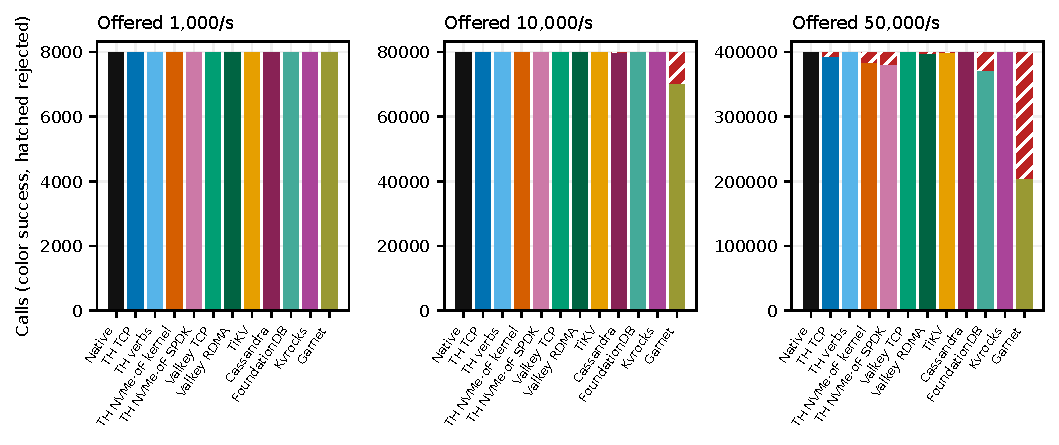
\includegraphics[width=.98\linewidth]{figures/offered.pdf}
\caption{Mixed 70/30 read/put offered load at 1~KiB, concurrency 32, 8~s per case: successful and rejected calls (\runs). Counts are not latency.}\label{fig:offered}
\end{figure}
No store rejects calls at 1,000 operations per second. At 10,000 per second Garnet rejects \N{rej:garnet:10000} calls and Cassandra \N{rej:cassandra:10000}. At 50,000 per second (400,000 calls) the rejected calls are: TH TCP \N{rej:th_tcp:50000}, NVMe-oF kernel \N{rej:th_kernel:50000}, NVMe-oF SPDK \N{rej:th_spdk:50000}, Valkey RDMA \N{rej:valkey_rdma:50000}, FoundationDB \N{rej:foundationdb:50000}, Garnet \N{rej:garnet:50000} and TiKV \N{rej:tikv:50000}. Native, TH verbs, Valkey TCP, Cassandra and Kvrocks reject none.

\begin{figure}[!htbp]\centering
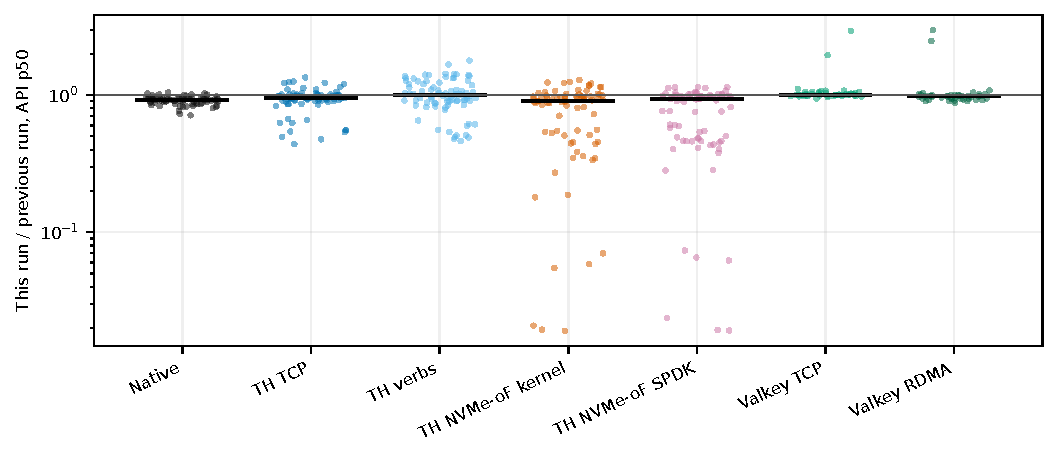
\includegraphics[width=.95\linewidth]{figures/crossrun.pdf}
\caption{This run against the previous campaign (\texttt{gcp-queue-bounded-campaign-20261106T032027Z}): API p50 ratio of each matched success population (\N{S:xr_common} populations). The black bar is the median per backend. Binary, queue policy and hosts differ between the runs. All stores use their final-run values here, not medians.}\label{fig:crossrun}
\end{figure}
Valkey did not change between the runs. Its median ratios are \N{S:xr_med:valkey_rdma|.2f} (RDMA) and \N{S:xr_med:valkey_tcp|.2f} (TCP), with 10th to 90th percentiles of \N{S:xr_p10:valkey_rdma|.2f} to \N{S:xr_p90:valkey_rdma|.2f} and \N{S:xr_p10:valkey_tcp|.2f} to \N{S:xr_p90:valkey_tcp|.2f}. This is the reproducibility of the fleet. Tidehunter over verbs has a median of \N{S:xr_med:th_verbs|.2f} and a spread of \N{S:xr_p10:th_verbs|.2f} to \N{S:xr_p90:th_verbs|.2f}. Its reads got slower (c16, 1~KiB: \N{old:p50:th_verbs:primary_rf1:read-concurrent:read:1024} to \RC{p50}{th_verbs}{1024}~\us; c1 mixed: \N{old:p50:th_verbs:primary_rf1:point-mixed:read:1024} to \PR{p50}{th_verbs}{1024}~\us). Its puts and 32-key reads got faster (put c16: \N{old:p50:th_verbs:primary_rf1:write-concurrent:put:1024} to \WC{p50}{th_verbs}{1024}~\us; 32-key read: \N{old:p50:th_verbs:primary_rf1:read-many32:get_many:1024} to \MR{p50}{th_verbs}{1024}~\us). The sealed 32-key repeat read at c16 on the kernel target fell from \N{old:p50:th_kernel:sealed_read:repeat_read-batch32-c16-baseline:get_many:1024} to \N{p50:th_kernel:sealed_read:repeat_read-batch32-c16-baseline:get_many:1024}~\us; the sealed initiator now requests 4 queues of depth 128 and earlier set no queue flags, but the cause is not isolated. The cause of the verbs read slowdown is not determined.

\section{Coherence of RDMA against TCP}\label{sec:coherence}
\begin{figure}[!htbp]\centering
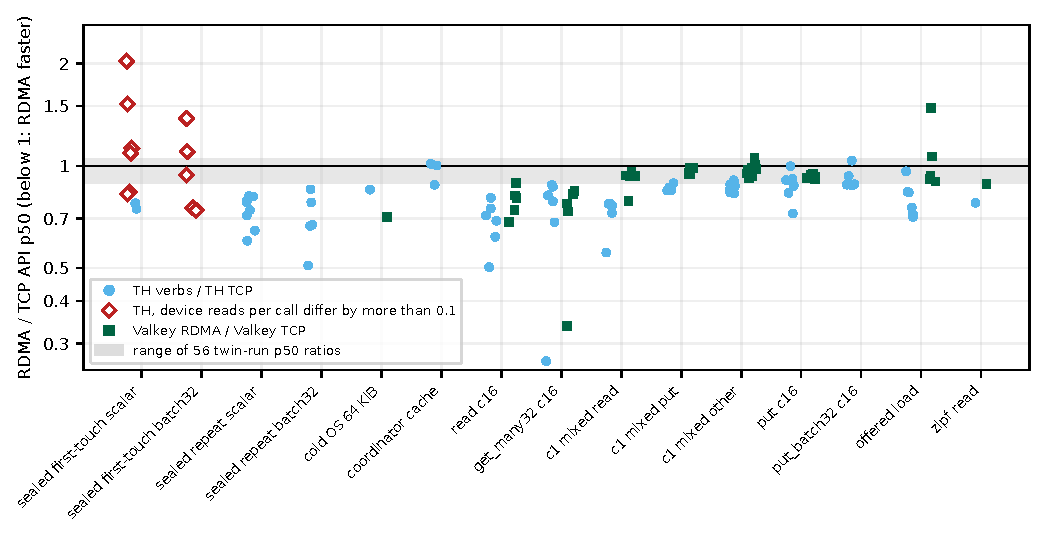
\includegraphics[width=.98\linewidth]{figures/coherence.pdf}
\caption{RDMA over TCP, API p50 ratio for \N{S:th_pairs} Tidehunter pairs (verbs over TCP) and \N{S:vk_pairs} Valkey pairs (RDMA over TCP), grouped by workload family. A pair has the same cohort, profile, value size, concurrency, operation, key count and offered rate. Red diamonds: the two Tidehunter paths differ by more than 0.1 device reads per call. The grey band is the range of the twin-run p50 ratios.}\label{fig:coherence}
\end{figure}
\textbf{p50.} Among the \N{S:th_pairs} Tidehunter pairs, verbs has a higher p50 than TCP in \N{S:th_p50_slower}. In \N{S:th_p50_slower_mismatch} of them the two paths read the SSD differently: first-touch scalar reads of 8~KiB (\N{ratio:p50:th_verbs/th_tcp:sealed_read:first_touch-scalar-c1-baseline:read:8192}$\times$; device reads per call \FT{dev}{th_verbs}{8192} for verbs and \FT{dev}{th_tcp}{8192} for TCP) and 64~KiB (\N{ratio:p50:th_verbs/th_tcp:sealed_read:first_touch-scalar-c1-baseline:read:65536}$\times$; \FT{dev}{th_verbs}{65536} and \FT{dev}{th_tcp}{65536}), plus four more first-touch cases. The other \N{S:th_p50_slower_tie} are ties of at most \N{S:th_p50_slower_tie_max|.2f}$\times$ (two coordinator-cache cases and one 8~KiB batch write). With matching device reads, verbs is lower in \N{S:th_matched_p50_faster} of \N{S:th_matched} pairs. In the repeat pass, where neither path reads an SSD, verbs is lower in all \N{S:th_repeat_pairs} pairs, by \N{S:th_repeat_ratio_lo|.2f} to \N{S:th_repeat_ratio_hi|.2f}$\times$.

\textbf{Why the device reads differ} is not determined. Both owners use the same read configuration (asynchronous member reads, four read workers, no resident-first read). The TCP, kernel and SPDK sealed cases share one physical dataset copy; verbs and Native have their own copies. The WAL file descriptor carries \texttt{POSIX\_FADV\_RANDOM} (\path{wal/mod.rs:408-431}), which turns off buffered read-ahead. A run of both transports on one copy, with block traces, would settle it.

\textbf{Tails.} Verbs p99 is above TCP p99 in \N{S:th_matched_p99_slower} of the \N{S:th_matched} pairs without device-read differences. Eleven are put, delete, missing-read or cache-hit cases with p99 ratios of 1.00 to 1.34. Two are first-touch reads of 64~B and 256~B: verbs p99 is \FT{p99}{th_verbs}{64} and \FT{p99}{th_verbs}{256}~\us\ against \FT{p99}{th_tcp}{64} and \FT{p99}{th_tcp}{256}~\us. The twin runs vary p99 by up to \N{S:twin_p99_hi|.1f}$\times$, so p99 inversions below a factor of two are not conclusive.

\textbf{Valkey.} RDMA is slower than TCP at p50 in \N{S:vk_p50_slower} of \N{S:vk_pairs} pairs (put at 1,000 operations per second, \N{ratio:p50:valkey_rdma/valkey_tcp:primary_rf1:offered-1000:put:1024}$\times$), at p99 in \N{S:vk_p99_slower} and at p99.9 in \N{S:vk_p999_slower}. The native \texttt{valkey-benchmark} controls show an RDMA p50 25 percent below TCP for GET (0.071 against 0.095~ms) and 38 percent below for SET (0.079 against 0.127~ms, published-as-written profile). Through the Rust adapter at c16 and 1~KiB the gain is \N{lower:p50:valkey_rdma/valkey_tcp:primary_rf1:read-concurrent:read:1024} percent for reads and \N{lower:p50:valkey_rdma/valkey_tcp:primary_rf1:write-concurrent:put:1024} percent for puts. \inference\ The client adapter absorbs part of the gain.

\section{Bottlenecks and next work}\label{sec:next}
This section ranks the bottlenecks that the data supports. The evidence is profiled twin cases (stage clocks overlap, so shares are indicative) and block-device counters. Each item names the next work and where it can run: \emph{local} means the laptop (TCP, local NVMe, no RDMA hardware); \emph{fleet} means the RDMA hardware is needed.
\begin{table}[!htbp]\centering
\small
\begin{tabular}{lrr}\toprule
Interval of one write call & mean \us & share\\\midrule
Caller entry, validation, admission & 9.2 & 2\%\\
\textbf{Wait in the command queue of the authority thread} & \textbf{63.5} & 17\%\\
Prepare and admit & 15.0 & 4\%\\
\textbf{Wait before append dispatch} & \textbf{65.5} & 17\%\\
Dispatch and transmit & 6.8 & 2\%\\
Append exchange with the owner & 105.3 & 27\%\\
\textbf{Wait for durable observation} & \textbf{69.1} & 18\%\\
Ordered publication & 24.7 & 6\%\\
Reply to the caller & 23.9 & 6\%\\
\midrule
Caller span (sum) & 383.1 & 100\%\\
\bottomrule\end{tabular}

\caption{Contiguous intervals between consecutive events of one instrumented write case (verbs, 1~KiB, concurrency 16, 4,096 calls, case 0491). Bold rows are waits. The intervals sum to the caller span. This twin run is instrumented; its span differs from the primary case.}\label{tab:timeline}
\end{table}
\begin{table}[!htbp]\centering
\small
\resizebox{\linewidth}{!}{%
\begin{tabular}{lrrrrrrrrr}\toprule
Case (8 KiB, c16) & calls & owners & total & pre-flight & group gap & admit & submit wait & flight & deliver + post\\\midrule
verbs, random keys (0474) & 222 & 4.7 & 892 & 134 & 116 & 66 & 265 & 149 & 161\\
TCP, random keys (0483) & 225 & 4.6 & 933 & 130 & 140 & 83 & 95 & 372 & 114\\
verbs, repeat batch (0095) & 226 & 4.8 & 729 & 114 & 136 & 59 & 183 & 170 & 68\\
verbs, sweep batch (0093) & 192 & 1.0 & 692 & 49 & 0 & 83 & 24 & 515 & 21\\
\bottomrule\end{tabular}}

\caption{Mean \us\ per traced 32-key call, on the path of the owner flight that finished last. Pre-flight: call start to the first flight's admission. Group gap: delay until the last flight's admission. Submit wait: admission to request submission. Flight: submission to completion. Owners is the mean number of owner flights per call. The traced calls are the first calls after the trace was armed.}\label{tab:readmany}
\end{table}
\begin{table}[!htbp]\centering
\small
\begin{tabular}{lrrrrr}\toprule
Store & p50 \us & writes/put (owners) & KiB/put (owners) & KiB/put (all hosts) & flushes/put\\\midrule
Native & 63.8 & 0.34 & 1.9 & 1.9 & 0.00\\
TH TCP & 322 & 0.54 & 13.2 & 17.8 & 0.00\\
TH verbs & 295 & 0.52 & 13.1 & 17.7 & 0.00\\
TH NVMe-oF kernel & 657 & 2.61 & 45.2 & 49.9 & 0.00\\
TH NVMe-oF SPDK & 702 & 2.57 & 44.2 & 49.0 & 0.00\\
Valkey TCP & 183 & 1.94 & 14.0 & 14.1 & 0.00\\
Valkey RDMA & 173 & 1.94 & 13.9 & 14.1 & 0.00\\
TiKV & 286 & 1.46 & 11.1 & 11.1 & 0.00\\
Cassandra & 263 & 1.29 & 9.2 & 9.4 & 0.00\\
FoundationDB & 986 & 0.13 & 4.2 & 6.5 & 0.00\\
Kvrocks & 262 & 3.00 & 17.1 & 17.5 & 0.00\\
Garnet & 144 & 0.94 & 4.9 & 5.0 & 0.00\\
\bottomrule\end{tabular}

\caption{Device writes of a 1~KiB put at concurrency 16 (synchronous tier; Native uses its value-WAL barrier). Writes and KiB per put are \texttt{/proc/diskstats} deltas of the Local SSD between the measurement gates, divided by successful puts. The owners columns use the five storage hosts (the coordinator\textquoteright s own SSD for Native); the all-hosts column adds the coordinator. They include journal, metadata and any other I/O on the device. Flushes are device flush requests. One repetition.}\label{tab:writes}
\end{table}
\begin{enumerate}[label=\textbf{B\arabic*.},leftmargin=2.2em]
\item \textbf{Write pipeline queueing at concurrency 16.} Affects every durable put (\N{ratio:p50:th_verbs/valkey_rdma:primary_rf1:write-concurrent:put:64} to \N{ratio:p50:th_verbs/valkey_rdma:primary_rf1:write-concurrent:put:65536}$\times$ Valkey RDMA).\\
\emph{Evidence.} At c1 the verbs put costs \PP{p50}{th_verbs}{1024}~\us, below Valkey RDMA (\PP{p50}{valkey_rdma}{1024}). At c16 it costs \WC{p50}{th_verbs}{1024}~\us. In the instrumented c16 case (Table~\ref{tab:timeline}) three waits add up to \N{S:tl_waits|.0f} of \N{S:tl_span|.0f}~\us\ (\N{S:tl_waits_pct|.0f} percent). The owner exchange takes \N{S:tl_exchange|.0f}~\us\ and contains the owner WAL fsync of \N{S:tl_walpersist|.0f}~\us\ (\N{S:tl_walpersist_pct|.0f} percent of the call). A durable receipt waited for earlier batches in \N{stagecount:0282:pre_completion_gate:write_durable_receipt_publication_blocked_batches} of \N{stagecount:0282:pre_completion_gate:write_durable_batches} batches. The owner appends \N{tlowner:batches_per_owner_record|.1f} batches per persist. All three waits are spent behind the coordinator authority thread (\texttt{wal-write-owner}). In one turn it takes up to 128 queued commands, then dispatches staged groups, accepts finished receipts and publishes (\path{concurrent.rs:1211-1217,1441}). Wait 1 grows with the commands queued ahead of it (Pearson $r=\N{tlcorr:w1}$). Waits 2 and 3 grow with the commands the thread takes in between ($r=\N{tlcorr:w2}$ and $\N{tlcorr:w3}$). Wait 2 averages \N{tlbucket:w2_competing0}~\us\ when the thread takes none and \N{tlbucket:w2_competing8}~\us\ when it takes eight; wait 3 averages \N{tlbucket:w3_competing0} and \N{tlbucket:w3_competing8}~\us.\\
\emph{Reading.} The fsync is not the bottleneck. \inference\ A staged group and a returned receipt wait for the next pipeline step of one thread that is busy admitting later commands. The preparation pool is not on this path (it serves \texttt{submit\_many}), and the durable result already travels in the owner response, so no second message can be removed. The counts are partly mechanical (a longer interval admits more events) and the trace adds overhead.\\
\emph{Next work (local, TCP).} A fixed bound on the commands one authority turn takes lowers waits 2 and 3 at c4 and c16, but it shrinks the owner group at c64 and lowers synchronous throughput there (laptop test of both tiers; \path{fixes/local-intake-ab/} of the analysis directory). Do not adopt a fixed bound. Test a bound that depends on free owner capacity. The queue-depth and wake counters at the three wait points now exist (the write-wait metrics of the G9 case in \path{docs/distributed/FOCUSED_CAMPAIGN_2026-11-07.md}); they have not run yet. Run them with a tracing-off control at c4, c16 and c64. Confirm on verbs.
\item \textbf{Live NVMe-oF write path.} \WC{p50}{th_kernel}{1024} and \WC{p50}{th_spdk}{1024}~\us\ at 1~KiB.\\
\emph{Evidence.} A live write is a reservation RPC, a remote write and a completion RPC. The initiator queue issues no flush; the owner persists after the completion (\path{live_io.rs:59-61}, \path{live_client.rs:320-345,430-503}). Stage means for the kernel case 0346 (SPDK case 0347 in brackets): control \N{stage:0346:live_nvmeof:control_ns} (\N{stage:0347:live_nvmeof:control_ns})~\us\ per exchange, two per write; persistence \N{stage:0346:live_nvmeof:persistence_ns} (\N{stage:0347:live_nvmeof:persistence_ns})~\us\ per write. The frontier file persistence (\N{stage:0346:live_nvmeof:frontier_file_ns} (\N{stage:0347:live_nvmeof:frontier_file_ns})~\us) and the frontier namespace persistence (\N{stage:0346:live_nvmeof:frontier_namespace_ns} (\N{stage:0347:live_nvmeof:frontier_namespace_ns})~\us) are nested in the persistence stage; the WAL persistence takes \N{stage:0346:live_nvmeof:wal_persistence_ns} (\N{stage:0347:live_nvmeof:wal_persistence_ns})~\us. The data transfer takes \N{stage:0346:live_nvmeof:cq_ns} (\N{stage:0347:live_nvmeof:cq_ns})~\us. The clocks overlap, so the stages do not add exactly. The owner RPC path persists the WAL file only (\N{stage:0282:profile:write_profile_storage_persist_wal_file_ns}~\us).\\
\emph{Reading.} The NVMe-oF data transfer is not the cost. The control exchanges and the frontier persistence are. The directory sync after the frontier rename protects the new root and cannot be skipped. Writes that complete together already share one persist, and the WAL directory sync runs only when a new WAL file starts (\path{storage.rs:2349-2479,3535-3602}); it did not run in these cases. At the device the live route writes \N{wrtk:th_kernel:primary_rf1:write-concurrent:put:1024}~KiB per 1~KiB put against \N{wrtk:th_verbs:primary_rf1:write-concurrent:put:1024}~KiB on the owner RPC (Table~\ref{tab:writes}); the counters do not say which files take the extra bytes. RF1 survives a restart with intact storage, not the loss of the owner or its Local SSD.\\
\emph{Next work (local).} Count how many writes share one persist on the current source and test that grouping with the existing crash tests. Merge the completion exchange of one group with the reservation of the next queued group (message change; needs approval). Do not persist the frontier at file rotation only: a crash could then drop acknowledged data. Keep writes on the owner RPC (hybrid route).
\item \textbf{32-key reads: coordinator time.} \N{ratio:p50:th_verbs/valkey_rdma:primary_rf1:read-many32:get_many:256} to \N{ratio:p50:th_verbs/valkey_rdma:primary_rf1:read-many32:get_many:64}$\times$ Valkey RDMA up to 1~KiB.\\
\emph{Evidence.} Table~\ref{tab:readmany}. A random 32-key call goes to \N{rm:0474:groups_per_call|.1f} owners. On verbs the owner flight is \N{rmpct:0474:flight_us} percent of the traced call (TCP: \N{rmpct:0483:flight_us} percent). The rest is coordinator time: pre-flight \N{rm:0474:preflight_us}~\us, group gap \N{rm:0474:group_gap_us}~\us\ (the delay from the first admission to the admission of the group that finished last), admission \N{rm:0474:admit_us}~\us\ and submit wait \N{rm:0474:submit_wait_us}~\us\ (TCP: \N{rm:0483:submit_wait_us}~\us). The pass already admits every group that fits and retires them in completion order (\path{pending_read.rs:331-450,454-542}), so the group gap does not show serial flights; in part of the traced calls a flight was submitted before the last group was admitted. A sweep batch to one owner has a flight share of \N{rmpct:0093:flight_us} percent.\\
\emph{Next work (local for dispatch and admission, fleet for the verbs submit wait).} Add trace events at dispatch and submission that separate credit shortage, a full lane and actor delay. Test starting a caller-owned lane inside the dispatch pass instead of in the finish loop (\path{pending_read.rs:454-489,3716-3750}). Sweep read lanes and pending-read credits one at a time. The cause of the verbs submit wait of \N{rm:0474:submit_wait_us}~\us\ is not determined.
\item \textbf{Owner cold-read path.} p50 \CO{p50}{th_verbs}{65536} to \CO{p50}{th_tcp}{65536}~\us\ against \CO{p50}{th_spdk}{65536} to \CO{p50}{th_kernel}{65536}~\us\ for NVMe-oF at 64~KiB.\\
\emph{Evidence.} \N{dev:th_tcp:cold_os_cache:cold-os-large:read:65536|.1f} device reads per call against \N{dev:th_kernel:cold_os_cache:cold-os-large:read:65536|.1f}, but only \N{devb:th_tcp:cold_os_cache:cold-os-large:read:65536}~bytes per call for a 65,536-byte value: the read is not split. The owner loaded authority history \N{stagecount:0448:authority:history_loads} times for 4,096 calls on TCP (\N{stagecount:0283:authority:history_loads} on verbs) against \N{stagecount:0348:authority:history_loads} (kernel) and \N{stagecount:0349:authority:history_loads} (SPDK) for NVMe-oF. A load reads small slots of the history files (\path{history.rs:15-18,202-207,480-503,581-615}) and the authority cache was full at 8,192 entries (\path{reference_directory.rs:26-29}). \inference\ The extra reads are these metadata reads. The counters do not attribute physical requests to files.\\
\emph{Next work (local, then fleet).} Trace block I/O with file attribution on a cold 64~KiB owner read to confirm. Then prewarm or widen the authority cache, or read the history path in fewer requests (persisted-format change; needs a decision). Until then route large cold reads over NVMe-oF.
\item \textbf{Coordinator cache capacity and policy.} A hit costs \CC{p50}{th_verbs}{256} to \CC{p50}{th_tcp}{8192}~\us\ against 32 to 610~\us\ for a miss.\\
\emph{Evidence.} Table~\ref{tab:hit}. The slot charge of at least 1~KiB limits the entry count.\\
\emph{Next work (local).} Exact per-entry charging is implemented and evaluated on synthetic and captured Sui traces. Measure a miss-ratio curve on a trace of real Sui objects (the mainnet checkpoint data gives object sizes and input-object locality, not a node KV trace) and compare admission policies.
\item \textbf{Read tails and stalls.} At concurrency 16 the verbs p99 is \RC{p99}{th_verbs}{1024} against a p50 of \RC{p50}{th_verbs}{1024}~\us\ (Valkey RDMA: \RC{p99}{valkey_rdma}{1024} against \RC{p50}{valkey_rdma}{1024}). The cold NVMe-oF cases stall for \N{p999ms:th_kernel:cold_os_cache:cold-os-large:read:65536} and \N{p999ms:th_spdk:cold_os_cache:cold-os-large:read:65536}~ms. First-touch reads of 64~B on verbs have a p99 of \FT{p99}{th_verbs}{64}~\us\ against \FT{p99}{th_tcp}{64}~\us\ on TCP. The causes are not determined.\\
\emph{Next work (fleet).} Trace the slowest calls of a profiled twin. Trace the start of a cold NVMe-oF case (connection state, first I/O after a cache drop). Compare progress-loop modes.
\item \textbf{Transport and client floor.} A small remote read costs about 30 to 40~\us\ on the owner RPC and the page-cache NVMe paths. On verbs the owner handler takes \N{stage:0041:profile:server_handler}~\us\ of an exchange of \N{stage:0041:profile:exchange}~\us\ (TCP: \N{stage:0011:profile:server_handler} of \N{stage:0011:profile:exchange}). An NVMe command takes \FT{initus}{th_kernel}{1024}~\us\ and the client adds \N{clientus:th_kernel:sealed_read:first_touch-scalar-c1-baseline:read:1024}~\us. This floor matters after B3 and B5. A cache hit removes it.
\item \textbf{Measurement gaps.} One repetition for Tidehunter and Native; the other stores are medians of earlier and current runs on different fleets. First-touch cases are not media-matched across transports. No CPU profile of the measured phase. No concurrency above 32. No NVMe/TCP. The 60 native-durability primaries did not run. Stage clocks overlap.\\
\emph{Next work.} Before another fleet run: record CPU per process for the measured phase only; run TCP and verbs on one physical dataset copy; add a direct-I/O control for the kernel target (needs a change of the owner lease check; not approved); repeat each focused case three times (the focused matrix has 270 and 324 cases; not run); add c64 and c256 (in the 324-case selection).
\end{enumerate}
\textbf{Order of work.} Start with B4 and B1 on the laptop. B4: a cold owner read with a block trace and a count of history loads. B1: the capacity-dependent bound. B3 needs tracing first. Add B5 with a Sui trace. Use the fleet to confirm B1 and B3 on verbs and to run B6 and B8. \inference\ The measured time in B1 and B3 is spent waiting, not in the SSD or on the wire, so gains are possible. The fixed-bound test shows that a simple change can trade latency for throughput.

\textbf{Do not pursue yet.} Do not tune NVMe-oF queue depth or build an SPDK initiator before B1 to B4: the NVMe command is \FT{initus}{th_kernel}{1024} to \FT{initus}{th_spdk}{1024}~\us\ of a \FT{p50}{th_kernel}{1024} to \FT{p50}{th_spdk}{1024}~\us\ read, and the SSD dominates when media is read. Do not send small writes over NVMe-oF. Do not compare transports on first-touch cases. Do not add Rust NVMe crates: none provides an NVMe-oF data path, and the existing \texttt{io-uring} and libfabric code covers the data plane.

\section{Provenance and limits}
Fleet \texttt{bench-0d99e8256fff4891} (parent run \texttt{bench-f12051ed5c6a42a8}). Binary \texttt{kv-research}: SHA-256 \path{4dcb94d54d0c3ca836ebacaf30e740fe4b6dff3d00483dc78c38dce460f114b7}. Package source tree: \path{aecddf26883ae80430197128b16c7cf815ae7967dfca1072f0fc87acd241d102}. The controller archive (983,653,857 bytes) matched the SHA-256 in the controller receipt (\path{660d3a109a11caff81a715c4f3c10ff309835949dceac83a049aeb041dc14979}). The fleet was deleted at 03:19 UTC. The per-object collection (16,465 objects) finished at 04:07 UTC. The results are in \path{gs://mysten-research-bench-artifacts/bench-0d99e8256fff4891/results/} and under \path{checkpoint-work/spdk-matched-storage-20261105T004442Z/gcp-full-matrix-campaign-20261106T213227Z-direct/}.

The gcloud login expired at 01:19 UTC and the launcher stopped. The guest controller kept running and exported its results. The suite started at 21:54 UTC and its work window ended at 03:02:47 UTC. The controller's own report step failed on the last case (\texttt{invalid live group storage persistence profile}). This brief uses the strict report regenerated with the fixed report code: 548 completed, 1 failed, 103 not run. The fixes made after this run are: a failed case no longer stops the report (a completed case is still checked strictly); the SPDK accounting check accepts the plain left-to-right sum for two derived means (the recorded values equal that sum, Python 3.12 sums floats with compensation, and the two values differed by $10^{-14}$~\us); the launcher keeps a 2-minute margin before VM expiry; and the launcher waits through a gcloud credential outage while it polls. The estimated compute cost is about \$114 (six hosts, 5.8 hours, \$3.29 per host-hour); it is an estimate, not an invoice.

Four native \texttt{valkey-benchmark} controls (published-as-written and matched-RAM profiles, TCP and RDMA) completed. They are histogram-based, not pooled with API populations. The inputs of this brief are in this directory: \path{build_inputs.py} reads the export and the table of cross-run medians of the other stores (\path{fixes/external-store-medians.csv} of the analysis directory) and writes \path{populations.csv}, \path{previous-populations.csv}, \path{device-reads.csv}, \path{write-timeline-spans.csv}, \path{readmany-trace.csv}, \path{stage-evidence.csv} and \path{external-spread.csv}. \path{plot_final.py} makes the figures and \path{evidence.json}. \path{make_tables.py} writes every number in this text from those tables. The timeline and read-trace tables are computed from the raw JSON. The other stage means come from \path{bottlenecks/stage-breakdown.csv} of the analysis directory; seven of them were checked against the raw JSON. No claim about Sui, physical NAND time, isolated network time or statistical significance follows from these measurements. The paper \cite{tidehunter} describes the single-node store. Its write acknowledgement does not wait for fsync (Section 3.1, ``Durability Guarantees''); the synchronous tier used here waits for a covering fsync. Native write latencies here are therefore not comparable with the paper's, and nothing in this brief contradicts the paper.

\begin{thebibliography}{9}\small
\bibitem{tidehunter} A. Chursin et al., \emph{Tidehunter: Large-Value Storage With Minimal Data Relocation}, \href{https://arxiv.org/abs/2602.01873v2}{arXiv:2602.01873v2}.
\end{thebibliography}
\clearpage
\appendix
\section{Full value-size tables}
Each entry is API p50/p99 in \us\ followed by successful calls/s. Primary live, native and Valkey cells are concurrency 16, RF1: scalar read $n=8{,}192$, scalar write $n=4{,}096$, 32-key calls $n=2{,}048$. Sealed rows are the first-touch c16 read cases; their media state differs from the live rows (Table~\ref{tab:media}). Sealed c16 cases exist for 1 KiB and 8 KiB only. A dash means no case, not zero. $^{*}$: the case ran, but its SPDK target counters are not admitted; the API latency is kept. One repetition.
\begin{table}[H]\centering\scriptsize\renewcommand{\arraystretch}{.88}\captionsetup{skip=1pt}
\resizebox{\linewidth}{!}{%
\begin{tabular}{lrrrr}\toprule
Backend & Scalar read & Scalar write & Read-many32 & Write-batch32\\\midrule
Native & 1.32/1.98/279{,}446 & 74.3/213/153{,}827 & 52.9/72.3/123{,}088 & 185/409/58{,}414\\
TH TCP & 57.2/210/176{,}727 & 323/536/48{,}408 & 808/1{,}945/18{,}061 & 1{,}488/2{,}204/10{,}219\\
TH verbs & 46.0/175/223{,}875 & 234/561/56{,}993 & 701/1{,}808/20{,}907 & 1{,}302/2{,}173/11{,}344\\
NVMe-oF kernel live & 56.2/253/165{,}298 & 646/1{,}216/24{,}264 & 644/3{,}000/18{,}291 & 1{,}701/2{,}698/8{,}968\\
NVMe-oF SPDK live & 75.0/157/146{,}998 & 697/1{,}382/22{,}430 & 644/2{,}718/18{,}600 & 1{,}818/2{,}818/8{,}599\\
Valkey TCP & 49.5/103/193{,}628 & 164/458/80{,}717 & 336/685/35{,}482 & --\\
Valkey RDMA & 44.1/89.2/211{,}858 & 152/357/86{,}852 & 283/819/40{,}614 & --\\
\bottomrule\end{tabular}}
\caption{64 B values: API p50/p99 (\us) / successful calls/s.}
\end{table}
\begin{table}[H]\centering\scriptsize\renewcommand{\arraystretch}{.88}\captionsetup{skip=1pt}
\resizebox{\linewidth}{!}{%
\begin{tabular}{lrrrr}\toprule
Backend & Scalar read & Scalar write & Read-many32 & Write-batch32\\\midrule
Native & 1.19/1.82/286{,}437 & 72.3/185/157{,}422 & 52.4/128/143{,}865 & 380/572/34{,}774\\
TH TCP & 60.4/213/169{,}009 & 321/540/47{,}723 & 797/1{,}956/18{,}111 & 1{,}683/2{,}647/9{,}297\\
TH verbs & 41.6/184/220{,}730 & 280/476/54{,}122 & 700/1{,}668/21{,}130 & 1{,}481/2{,}433/10{,}386\\
NVMe-oF kernel live & 49.4/195/144{,}489 & 647/1{,}344/23{,}890 & 634/2{,}926/18{,}328 & 1{,}728/2{,}885/8{,}464\\
NVMe-oF SPDK live & 69.4/150/145{,}562 & 703/1{,}266/22{,}293 & 661/2{,}597/18{,}537 & 2{,}116/3{,}097/7{,}566\\
Valkey TCP & 52.0/103/192{,}026 & 173/439/78{,}863 & 376/784/32{,}058 & --\\
Valkey RDMA & 42.5/87.4/165{,}415 & 158/359/87{,}818 & 291/806/39{,}895 & --\\
\bottomrule\end{tabular}}
\caption{256 B values: API p50/p99 (\us) / successful calls/s.}
\end{table}
\begin{table}[H]\centering\scriptsize\renewcommand{\arraystretch}{.88}\captionsetup{skip=1pt}
\resizebox{\linewidth}{!}{%
\begin{tabular}{lrrrr}\toprule
Backend & Scalar read & Scalar write & Read-many32 & Write-batch32\\\midrule
Native & 1.37/2.18/277{,}534 & 63.8/168/168{,}290 & 55.3/113/110{,}340 & 1{,}047/1{,}247/13{,}901\\
TH TCP & 60.1/209/172{,}074 & 322/506/47{,}427 & 840/2{,}418/16{,}895 & 2{,}554/3{,}576/6{,}363\\
TH verbs & 45.0/176/220{,}750 & 295/575/51{,}467 & 688/1{,}723/19{,}913 & 2{,}256/3{,}212/7{,}191\\
NVMe-oF kernel live & 55.9/242/181{,}799 & 657/1{,}206/23{,}841 & 641/2{,}846/18{,}272 & 2{,}421/3{,}810/6{,}322\\
NVMe-oF kernel sealed & 98.1/267/136{,}837 & -- & 558/1{,}347/25{,}693 & --\\
NVMe-oF SPDK live & 71.7/156/147{,}290 & 702/1{,}248/22{,}172 & 642/2{,}740/18{,}391 & 2{,}253/4{,}030/6{,}405\\
NVMe-oF SPDK sealed & 116/173/123{,}479 & -- & 567/1{,}104/25{,}664 & --\\
Valkey TCP & 53.4/113/188{,}256 & 183/469/73{,}443 & 389/807/29{,}860 & --\\
Valkey RDMA & 43.1/92.5/165{,}026 & 173/410/80{,}146 & 321/803/35{,}821 & --\\
\bottomrule\end{tabular}}
\caption{1 KiB values: API p50/p99 (\us) / successful calls/s.}
\end{table}
\begin{table}[H]\centering\scriptsize\renewcommand{\arraystretch}{.88}\captionsetup{skip=1pt}
\resizebox{\linewidth}{!}{%
\begin{tabular}{lrrrr}\toprule
Backend & Scalar read & Scalar write & Read-many32 & Write-batch32\\\midrule
Native & 2.55/4.01/267{,}273 & 208/380/67{,}505 & 72.1/266/52{,}852 & 10{,}807/12{,}943/1{,}506\\
TH TCP & 77.6/260/135{,}957 & 474/1{,}120/30{,}822 & 874/1{,}728/14{,}522 & 7{,}387/14{,}042/2{,}006\\
TH verbs & 47.9/163/201{,}670 & 473/1{,}012/31{,}152 & 595/1{,}586/19{,}090 & 7{,}654/12{,}549/2{,}066\\
NVMe-oF kernel live & 60.7/211/140{,}976 & 888/1{,}779/17{,}294 & 630/2{,}228/17{,}072 & 6{,}358/12{,}856/2{,}338\\
NVMe-oF kernel sealed & 102/482/121{,}803 & -- & 451/1{,}142/23{,}612 & --\\
NVMe-oF SPDK live & 112/162/127{,}916 & 971/1{,}972/15{,}680 & 639/2{,}055/17{,}064 & 7{,}777/16{,}285/1{,}850\\
NVMe-oF SPDK sealed & 129/300/106{,}573 & -- & 492/1{,}044/22{,}895 & --\\
Valkey TCP & 67.1/149/149{,}011 & 229/575/59{,}373 & 512/202{,}686/2{,}926 & --\\
Valkey RDMA & 45.9/82.0/142{,}170 & 217/521/63{,}414 & 375/1{,}149/21{,}097 & --\\
\bottomrule\end{tabular}}
\caption{8 KiB values: API p50/p99 (\us) / successful calls/s.}
\end{table}
\begin{table}[H]\centering\scriptsize\renewcommand{\arraystretch}{.88}\captionsetup{skip=1pt}
\resizebox{\linewidth}{!}{%
\begin{tabular}{lrrrr}\toprule
Backend & Scalar read & Scalar write & Read-many32 & Write-batch32\\\midrule
Native & 14.8/24.7/226{,}188 & 2{,}714/3{,}337/6{,}102 & 1{,}145/45{,}168/2{,}915 & 57{,}850/68{,}469/269\\
TH TCP & 165/641/60{,}472 & 1{,}611/3{,}321/9{,}093 & 5{,}737/209{,}166/949 & 36{,}579/55{,}357/444\\
TH verbs & 83.1/290/102{,}653 & 1{,}463/3{,}984/9{,}937 & 1{,}524/33{,}235/3{,}927 & 34{,}144/49{,}677/476\\
NVMe-oF kernel live & 76.5/150/110{,}105 & 1{,}802/5{,}023/7{,}588 & 1{,}262/31{,}236/4{,}498 & 46{,}208/282{,}869/265\\
NVMe-oF SPDK live & 147/218/83{,}412 & 2{,}146/6{,}429/6{,}284 & 1{,}278/29{,}600/4{,}872 & 59{,}404/551{,}174/180\\
Valkey TCP & 157/657/53{,}251 & 455/1{,}256/28{,}957 & 4{,}265/213{,}368/265 & --\\
Valkey RDMA & 116/276/72{,}961 & 419/1{,}120/31{,}902 & 1{,}440/43{,}334/2{,}159 & --\\
\bottomrule\end{tabular}}
\caption{64 KiB values: API p50/p99 (\us) / successful calls/s.}
\end{table}

\end{document}
